\documentclass[11pt,a4paper,oneside]{book}

\usepackage[english]{babel}

%%\usepackage{times}
\usepackage{helvet}
\renewcommand*\familydefault{\sfdefault} %% Only if the base font of the

\usepackage[T1]{fontenc}
\usepackage[latin1]{inputenc}
\usepackage{amsmath}
\usepackage{amssymb}
\usepackage{graphicx}
\usepackage{longtable}
\usepackage{multirow}
\usepackage{tabularx}
\usepackage{fancyhdr}
\usepackage{float}
\usepackage[Sonny]{fncychap}
\usepackage{hyperref} % Indice nel pdf, da togliere per la stampa perché crea conflitto.
\usepackage{subfigure}
\usepackage{pdfpages}
\usepackage{titlesec}
\usepackage{rotating}
\usepackage{color}
\usepackage{gensymb}
\usepackage{fixltx2e}
\usepackage[citestyle=numeric,hyperref,natbib=true,backend=bibtex]{biblatex}
\renewcommand\nameyeardelim{, }


%\addbibresource{Bibliografia}
%\pagestyle{empty}

\usepackage{geometry}
 \geometry{
 a4paper,
 total={210mm,297mm},
 left=30mm,
 right=35mm,
 top=30mm,
 bottom=40mm,
 }


\newcommand{\tb}{\textsubscript}
\newcommand{\ts}{\textsuperscript}

\graphicspath{{./immagini/}}


\begin{document}


%\begin{titlepage}
\thispagestyle{empty}


\begin{center}
\text{\large Institute for Renewable Energy}
\end{center}

\begin{figure}[h]
     \begin{center}
         
\includegraphics[width=0.5\textwidth]{logo}
     \end{center}
     \label{fig:logo_uni}
 \end{figure}

\vspace{4 cm}

\begin{center} 
%\text{\LARGE Usefulness of Landsat data for monitoring vegetation changes}\\
\text{\Huge  TypeDLT}\\
\vspace{0.5 cm}
\text{\Huge Tutorial}\\

\end{center}

%\vspace{1.2 cm} 
% %\rule{1.0\textwidth}{0.5pt}
%\hrule \
%\vspace{0.5 cm}
% \begin{center}
%\textsc{3D Finite Volume Method applied to Heat-Transfer}\\
%\end{center}
%\hrulefill \

\vspace{5 cm}

\begin{tabular}{lr}  
 
Contacts	&			\\

Giuseppe De Michele		& \href{mailto:giuseppe.demichele@eurac.edu}{giuseppe.demichele@eurac.edu}	 			\\
Ulrich Filippi Oberegger		&	\href{mailto:ulrich.filippi@eurac.edu}{ulrich.filippi@eurac.edu}				\\
Luca Baglivo 		&		\href{mailto:luca.baglivo@eurac.edu}{luca.baglivo@eurac.edu}			\\
\end{tabular}

\end{titlepage}


%DA DECOMMENTARE AL MOMENTO DELLA STAMPA INTEGRALE
%\newpage
%\null
%\thispagestyle{empty}
%\newpage

\pagestyle{fancy} 
\fancyhf{}%cancella tutti i campi 
%\headsep 2cm %altrimenti si sovrappone il testo alla hdr 
\fancyhead[R]{\includegraphics*[width=3cm]{logo}% non c'è l'ambiente figure.
} 
\fancyhead[L]{\large \textsc{TypeDLT - Tutorial} }
\fancyfoot[C]{\thepage}
\renewcommand{\headrulewidth}{0.1pt}


%\listoffigures
%\listoftables

%\input{chapter/sommario}


%\mainmatter
\begin{titlepage}
\thispagestyle{empty}


\begin{center}
\text{\large Institute for Renewable Energy}
\end{center}

\begin{figure}[h]
     \begin{center}
         
\includegraphics[width=0.5\textwidth]{logo}
     \end{center}
     \label{fig:logo_uni}
 \end{figure}

\vspace{4 cm}

\begin{center} 
%\text{\LARGE Usefulness of Landsat data for monitoring vegetation changes}\\
\text{\Huge  TypeDLT}\\
\vspace{0.5 cm}
\text{\Huge Tutorial}\\

\end{center}

%\vspace{1.2 cm} 
% %\rule{1.0\textwidth}{0.5pt}
%\hrule \
%\vspace{0.5 cm}
% \begin{center}
%\textsc{3D Finite Volume Method applied to Heat-Transfer}\\
%\end{center}
%\hrulefill \

\vspace{5 cm}

\begin{tabular}{lr}  
 
Contacts	&			\\

Giuseppe De Michele		& \href{mailto:giuseppe.demichele@eurac.edu}{giuseppe.demichele@eurac.edu}	 			\\
Ulrich Filippi Oberegger		&	\href{mailto:ulrich.filippi@eurac.edu}{ulrich.filippi@eurac.edu}				\\
Luca Baglivo 		&		\href{mailto:luca.baglivo@eurac.edu}{luca.baglivo@eurac.edu}			\\
\end{tabular}

\end{titlepage}


\tableofcontents

\chapter*{Introduction}
TypeDLT is a new component for TRNSYS able to perform daylighting simulation of complex fenestration system using RADIANCE. The new type has been developed by the Institute of Renewable Energy of EURAC within the EU FP7 Project CommONEnergy. \\
The TypeDLT expand the capabilities of TRNSYS allowing to take in account also the visual comfort in order to have a overall vision of the behaviour of the building in terms of energy balance but also thermal and visual comfort. It is also possible the connection of TypeDLT with other types on the TRNSYS deck in order to define custom shading controls. 
\\
\\
The following document explain how to start with the daylighting simulation within TRNSYS. 
\chapter{Creating a simple model}
First, it is necessary to download and install the following software:

\begin{itemize}
\renewcommand{\labelitemi}{\tiny$\blacksquare$}
\item Google SketchUp from \url{http://www.sketchup.com/}
\item su2rad (version 2014.0.0) from \url{https://github.com/tbleicher/su2rad}
\end{itemize}

Once installed the software and chosen the template ('Engineering - Meters')  the screen in SketchUp will appear as in figure \ref{img1:su2rad}, where in the Plugins section it is possible to find the Radiance one.

\begin{figure}[H]
\centering
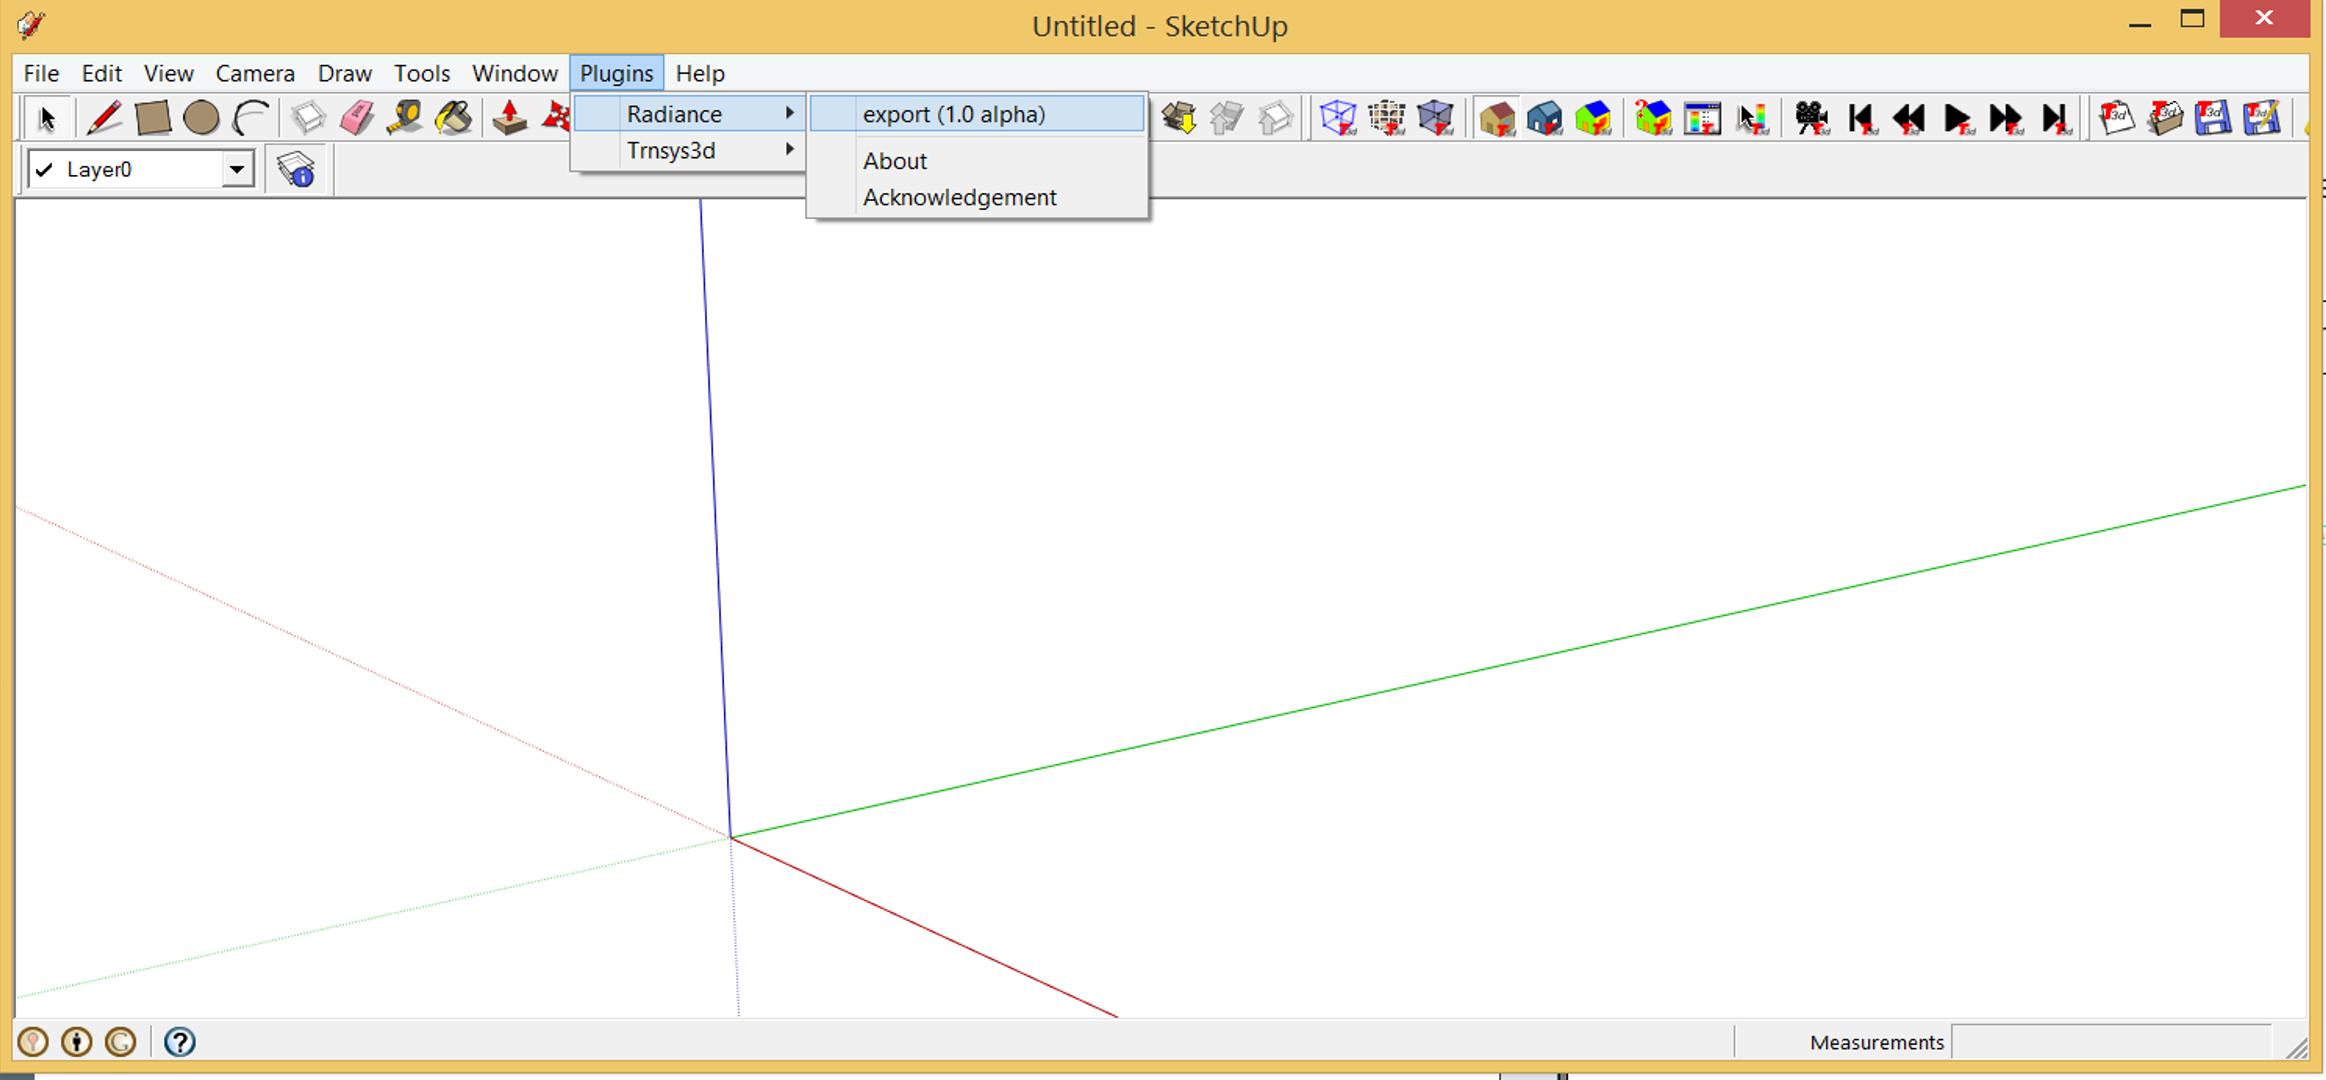
\includegraphics[width=0.9\textwidth]{su2rad}
\caption{\label{img1:su2rad} Initial screen in SketchUp with su2rad installed}
\end{figure}

\section{Draw a model}

Draw a model is very simple thanks to the user-friendly interface and the tools of SketchUp. As example we will create a shoe-box with an opening for the window on the south side of dimension 5x8x2.7 m. First, it is necessary to draw a horizontal surface that will be the plan of our box with the \textit{Rectangle} tool and then extrude this surface with the \textit{Push/Pull} tool, giving the third dimension to the box. The box will appear as the one in figure \ref{img1:box}. The orientation of the cardinal points as recognized by Radiance are also shown in the figure \ref{img1:su2rad}, the north-south direction is on the green axis  and east-west on the red axis. The blue axis points toward the sky.

\begin{figure}[h]
\centering
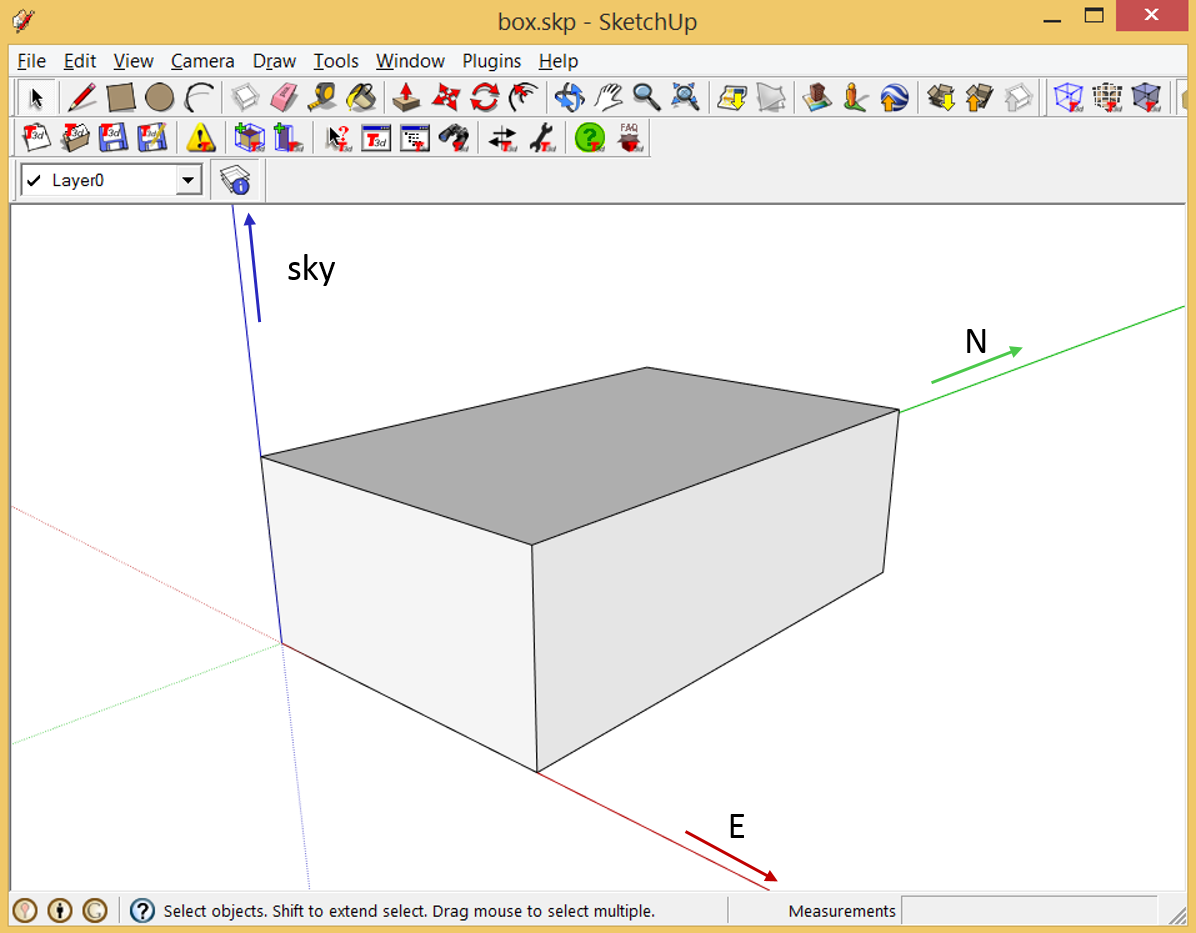
\includegraphics[width=0.9\textwidth]{box2}
\caption{\label{img1:box} Shoe-box drawn in SketchUp}
\end{figure}

Now it is necessary to draw the window on the south fa\c{c}ade. Select the \textit{Rectangle} tool and draw a rectangle on the vertical surface of dimension 3x1.2 m, distant 1 m from the side corner and 0.9 m from bottom. At this point assign a material to this new surface, open the \textit{Paint Bucket} and select a translucent glass material and click on the window surface. This step is not strictly required just because the material are set in a second phase, but it is useful to find easily the window in scene and have a overall idea of the geometry. Add also a ground surface to the scene, again using the \textit{Rectangle} tool. The box in figure \ref{img1:boxWin} is obtained. 

\begin{figure}[h]
\centering
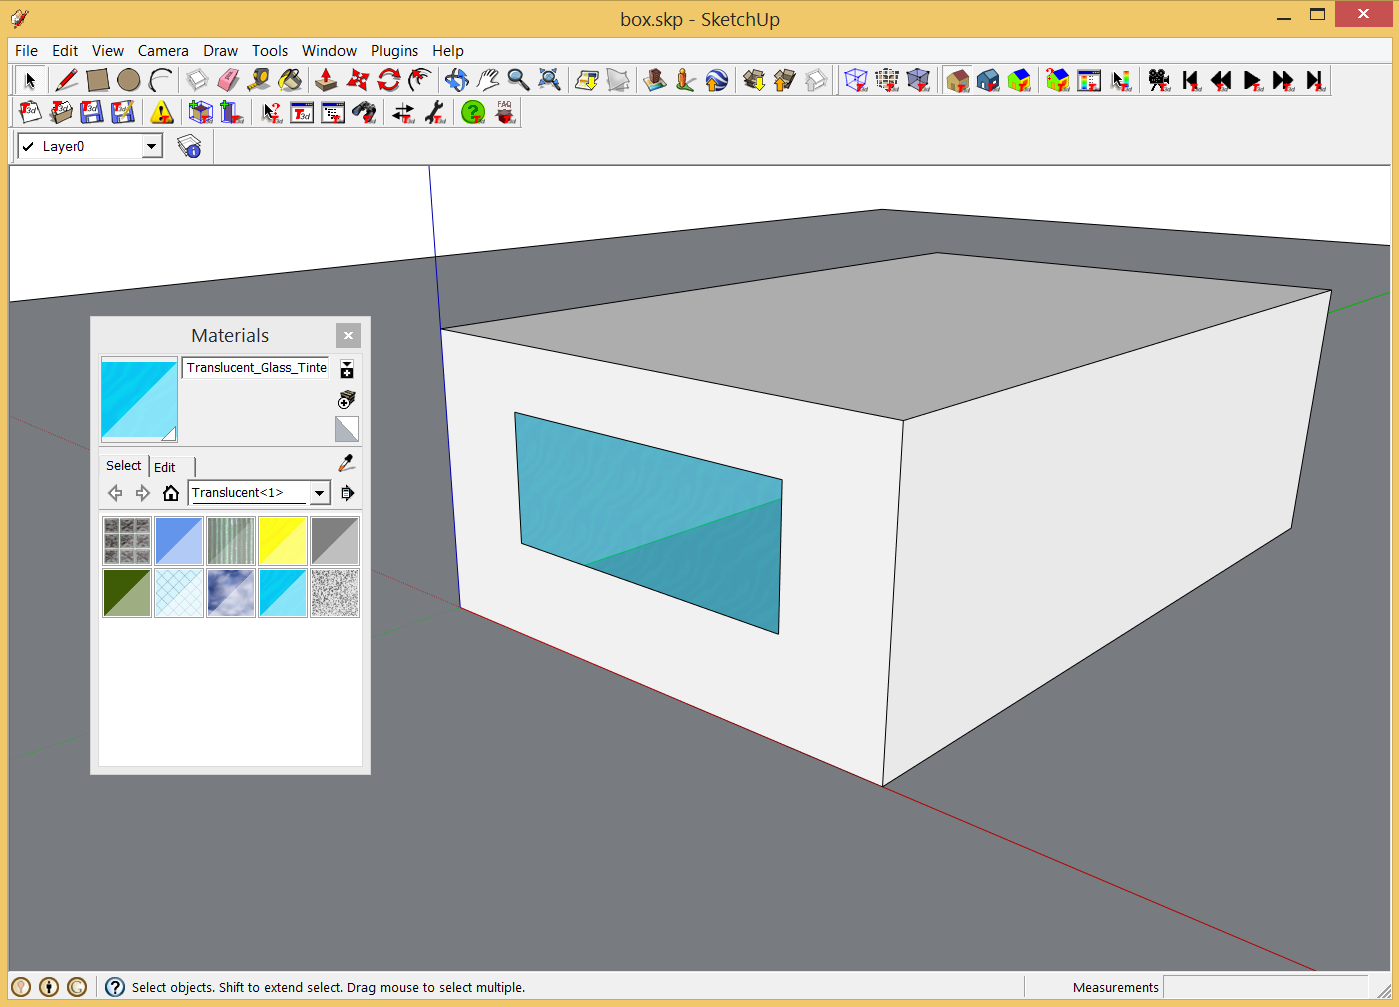
\includegraphics[width=0.9\textwidth]{boxWin2}
\caption{\label{img1:boxWin} Shoe-box with window on south fa\c{c}ade}
\end{figure}

Once the geometry is complete, the materials for each group of component has to be assigned. Assign at each layer a material and collect in each layer the surfaces with the same material/reflectance factor. This method allows to change very easily the material within Radiance. To do this open the layer window from \textit{Window -> Layers} and add as many layer as required by clicking on the "+" button. The common approach is set the layer as the main elements of the building that have the same reflectance: internal walls, 
external walls, ceiling, floor, Windows, ground, etc. Do not let space between the words in the name of the layer (i.e. layer Internal walls became Internal\_walls).

The procedure to move one or more surfaces from one layer to another is:
\begin{enumerate}
\item Select one or more surfaces. The selected entities are highlighted as dotted surfaces.
\item Activate the context menu for the selected entities, right click of the mouse.
\item Select the \textit{Entity Info} menu item. The Entity Info dialog box appears.
\item Select the layer for the entities from the 'Layers' drop-down list, figure \ref{img1:layer}.
\end{enumerate}

After moved all the surfaces in the respective layers, export the geometry created in a Radiance geometry. Before to export, place the view into the room and direct it toward the window (figure \ref{img1:inside}). This will be export in a Radiance view file that is useful to check if the window surface normal faces into the room (see section \ref{sec:normalsurf}). \\


\begin{figure}[h]
\centering
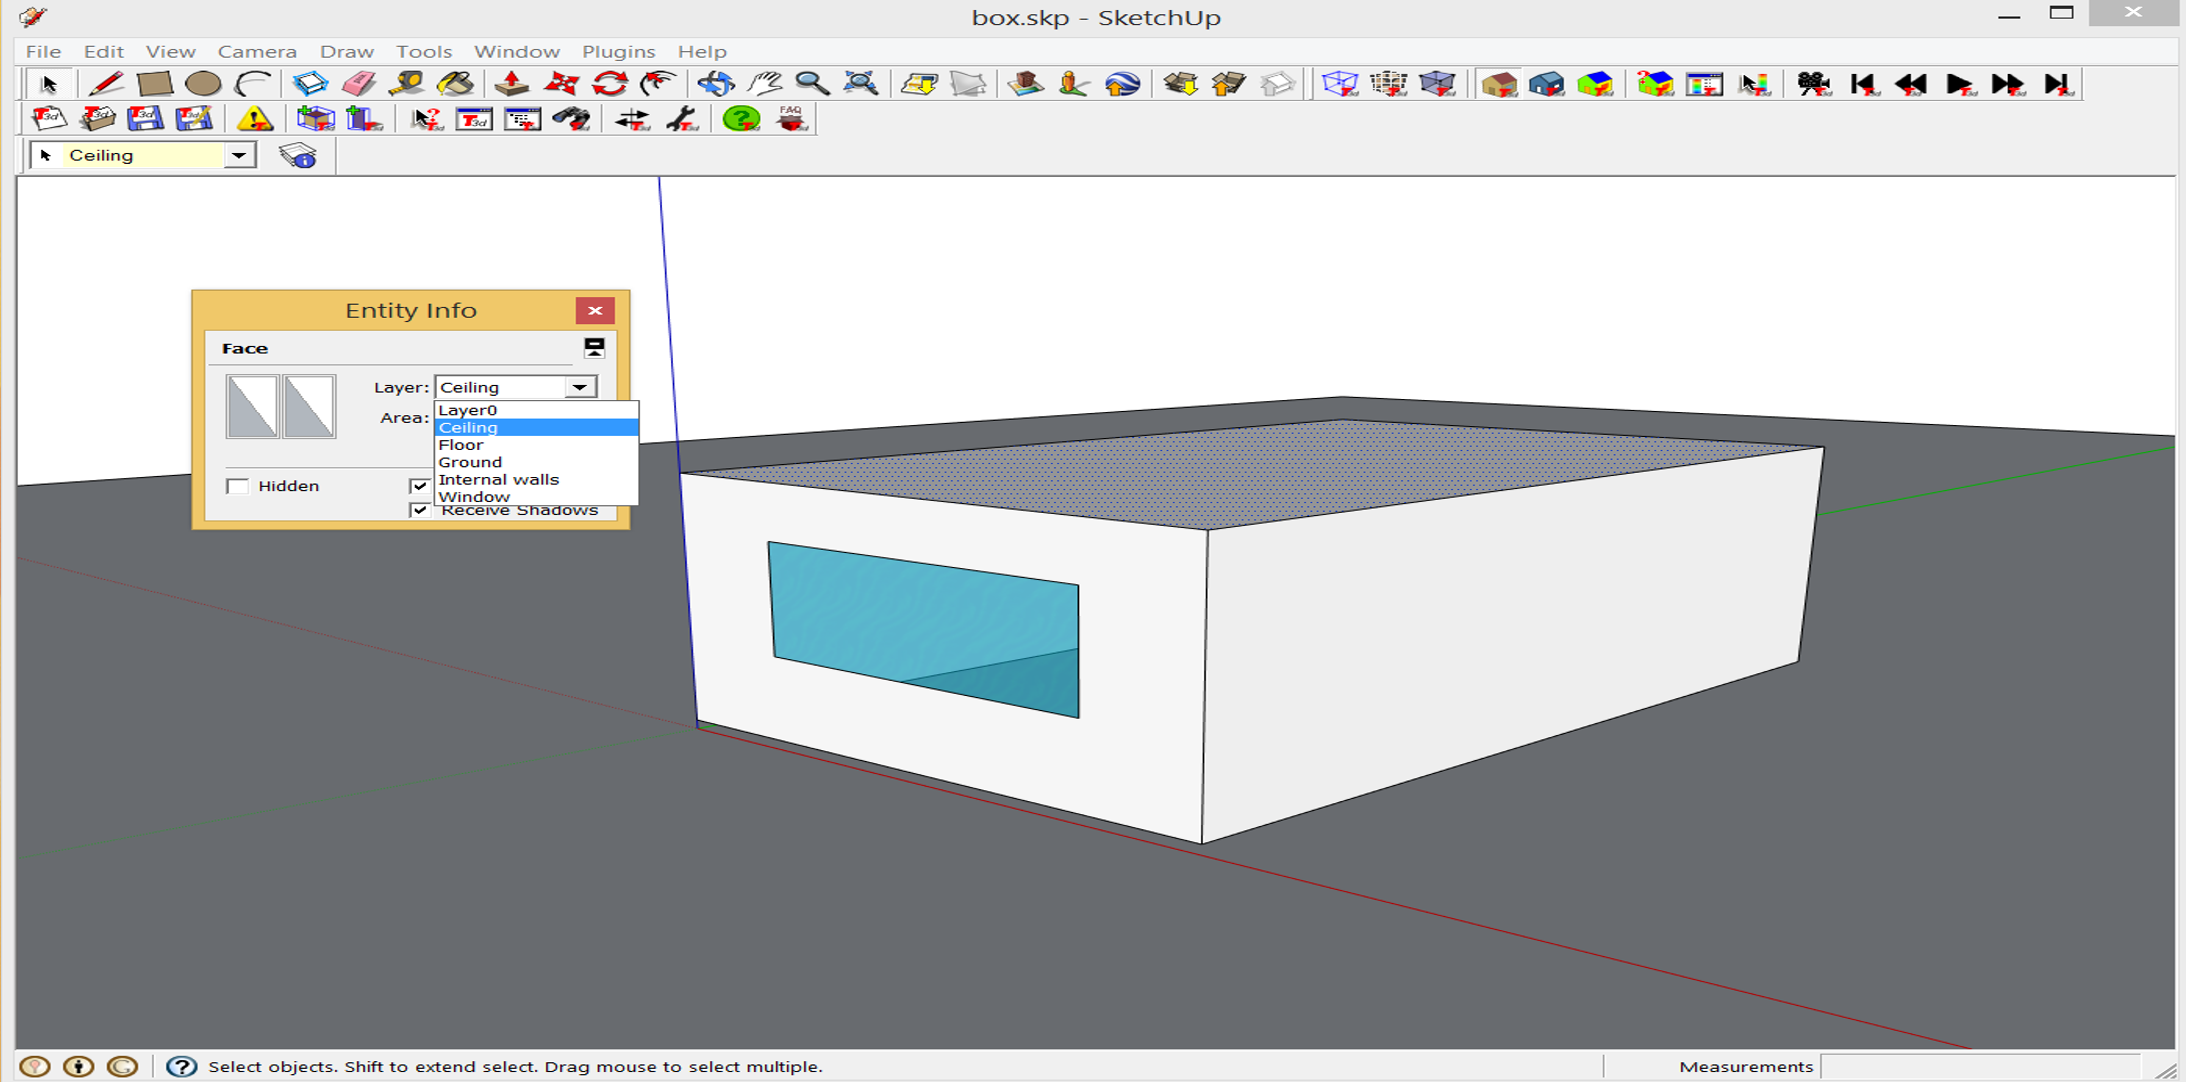
\includegraphics[width=0.9\textwidth]{layer}
\caption{\label{img1:layer} Definition of the surface in the respective layer}
\end{figure}


\begin{figure}[H]
\centering
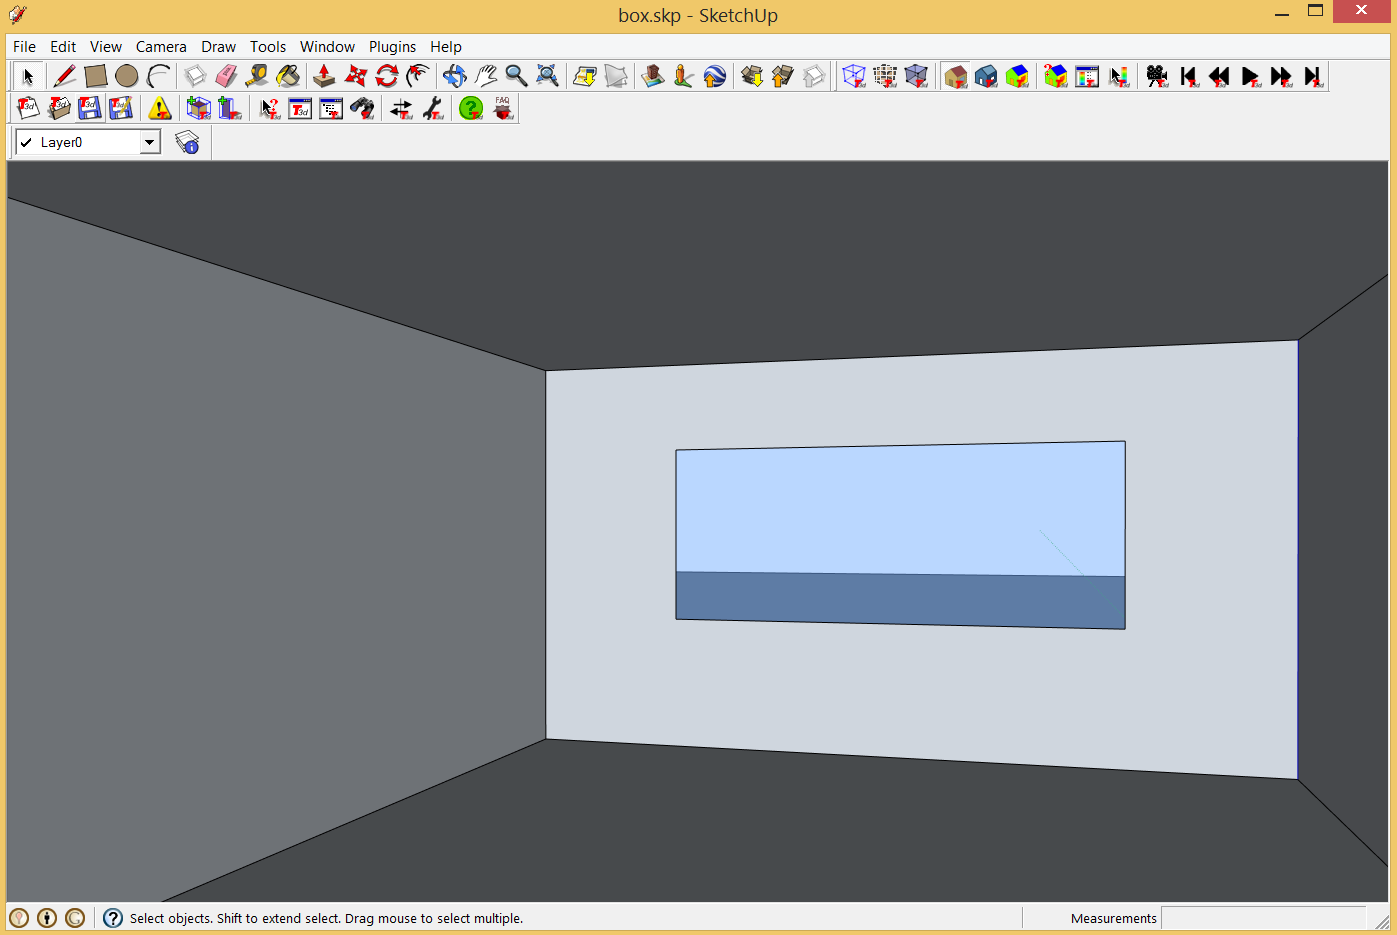
\includegraphics[width=0.9\textwidth]{insideview}
\caption{\label{img1:inside} View inside that will be used to check the direction of the window surface normal}
\end{figure}

\section{Export the model with su2rad} \label{sec:export}

Now export the Radiance geometry, open the su2rad export menu \textit{Plugins -> Radiance -> Export} (figure \ref{img1:export_menu}). Between the several windows available, you have to work on \textit{Export} (figure \ref{img1:export}), in which it is possible to define the path, the name of the scene and the mode. The name of the scene has to be defined considering the ID of the zone, that will be also the name of the folder containing the Radiance files (e.g. Zone1), see section \ref{sec:manualtweaks}. Regarding the exportation mode, case select "by layer" from the drop-down list. On the window \textit{Materials} (figure \ref{img1:materials}) the material for each layer can be set. \\
The SketchUp materials are displayed in three different ways:
\begin{itemize}
\renewcommand{\labelitemi}{\tiny$\blacksquare$}
\item Materials without corresponding names in the Radiance library are yellowish-brown. If there is no alias assigned to them for the export there will be a simple conversion of the SketchUp color.
\item Materials with corresponding names in the library are displayed in blue. They are exported with the definition from the library unless they are assigned another material.
\item Materials that have been assigned a Radiance definition are blue, too, and show the definition below the name. The definition from the library will be copied to the "materials.rad" file and an alias for the SketchUp material name will be added.
\end{itemize}
In order to assign a material to a SketchUp material/layer select the materials from the right column and drag it over the material/layer to the left. The color of the SketchUp material/layer will change to a darker shade and if you replace an existing material it will be outlined in red.
Below the two list of materials and layers, a window shows the definition of the Radiance material.

\begin{figure}[h] 
  \subfigure[Export menu]{% 
    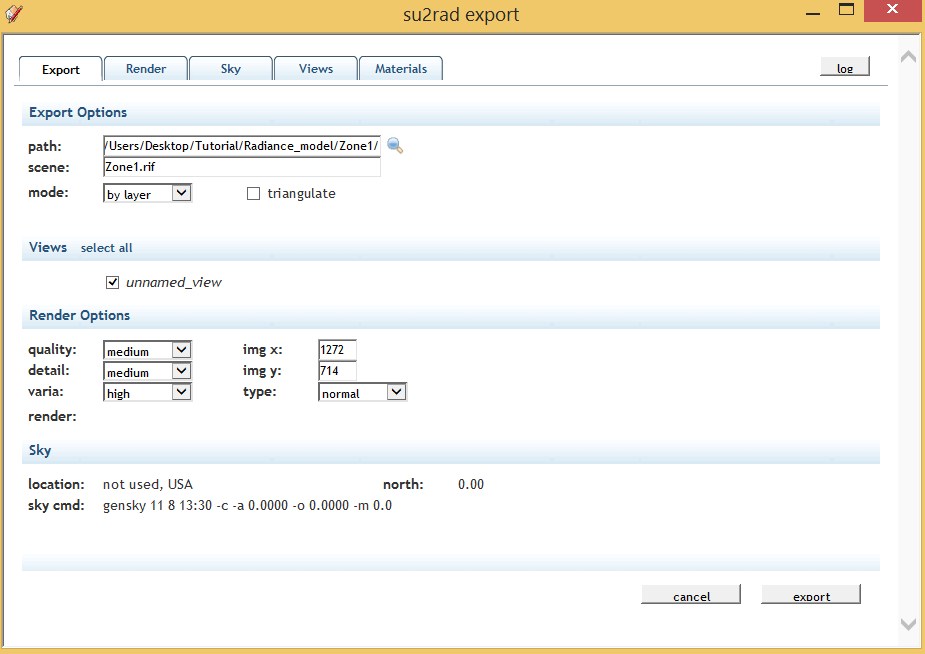
\includegraphics[width=.49\textwidth]{export2} \label{img1:export} 
  }
  \subfigure[Materials menu]{% 
    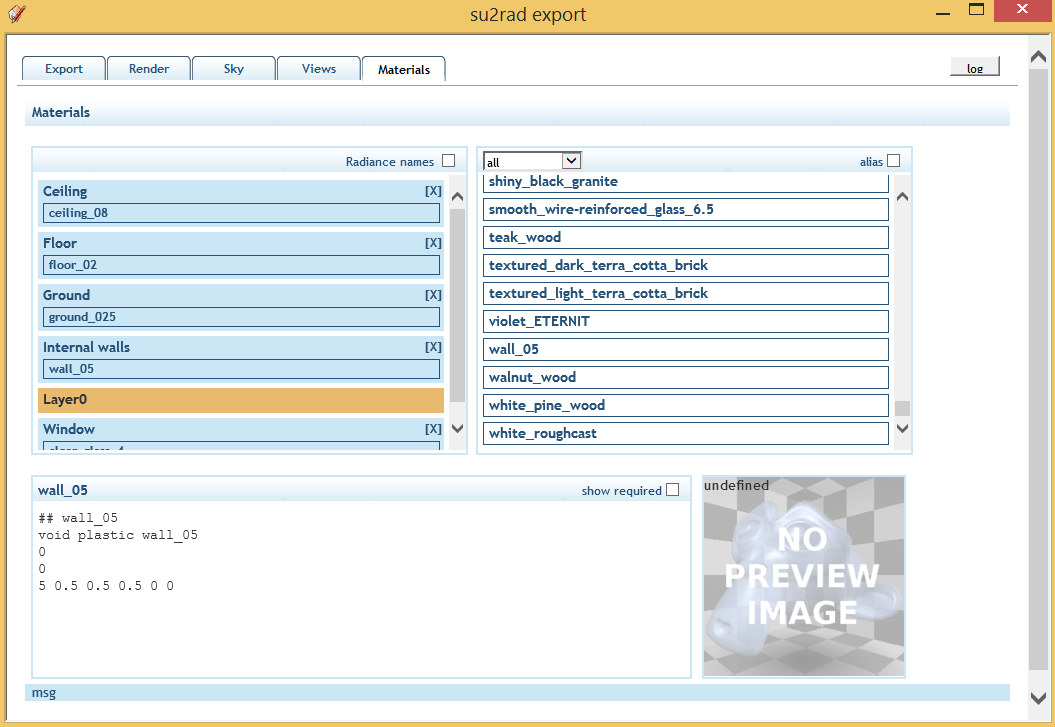
\includegraphics[width=.51\textwidth]{materials} \label{img1:materials} 
  } 
  \caption{\label{img1:export_menu} su2rad export options}
\end{figure}

Once all is set-up, export in Radiance geometry by clinking on export (figure \ref{img1:export}). In the path previously defined a new folder containing the new geometry will be created.

\begin{figure}[h]
\centering
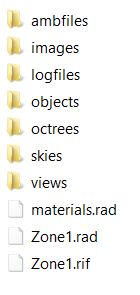
\includegraphics[width=0.2\textwidth]{exported}
\caption{\label{img1:exported} Contents of the folder export with su2rad}
\end{figure}


\subsection{Defining Custom Radiance Materials}
Probably, the default materials of su2rad are not useful for the user, therefore defining custom material became necessary. The ways to define custom materials are two:
\begin{enumerate}
\item adding the material to the su2rad library and assign it directly in SketchUp
\item creating the material manually and connecting it to the layer after the su2rad exportation
\end{enumerate}
First option allows also to reuse the material created for other models. 
In both cases the definition of the material has to respect the following syntax 
\begin{flalign*}
&<mod> <primitive> <id>\\
&<nargs> [args]\\
&<nargs> [args]\\
&<nargs> [args]\\
\end{flalign*}
The different definition of primitives and arguments depend of the material type, a deeper explanation and example of materials can be found in \url{http://radsite.lbl.gov/radiance/refer/ray.html#Materials} and \url{http://www.artifice.com/radiance/rad_materials.html}. \\
A useful tool for creating Radiance plastic and metal materials and seeing an high-quality preview of the material created is \textit{Radiance Colour Piker}, available at \url{http://www.jaloxa.eu/resources/radiance/colour_picker.shtml} by clicking on the button \textit{Launch the Colour Picker}. Once the material is generated, it can be copy and paste in the materials definition of Radiance scene.
\paragraph{Adding material in the su2rad material library}
Adding a material to the su2rad library is quite simple. First, move in the su2rad plungins folder and open the folder \textit{ray}, usually the path where find the folder is \textit{C:\textbackslash Program Files (x86)\textbackslash Google\textbackslash Google SketchUp 8\textbackslash Plugins\textbackslash su2radlib\textbackslash ray}.\\
Within the ray folder are present three file:
\begin{itemize}
\renewcommand{\labelitemi}{\tiny$\blacksquare$}
\item K\_and\_E.rad
\item  ral.rad
\item materials.rad
\end{itemize}
where ral.rad and K\_and\_E.rad contain materials corresponding to specific colour scales. Materials.rad contains more realistic material (e.g. wood, concrete, etc.). The latter file is the one that has to be modified. Before modifying the file, create a backup copy of it and rename as \textit{materials\_orginal.rad}.\\
Open the material.rad with notepad (or equivalent software) and add at the bottom of the file the material just created. In figure \ref{img1:materialrad} has been also created a section within the file called "My materials" useful to identify immediately where the custom materials are located.
\begin{figure}[h]
\centering
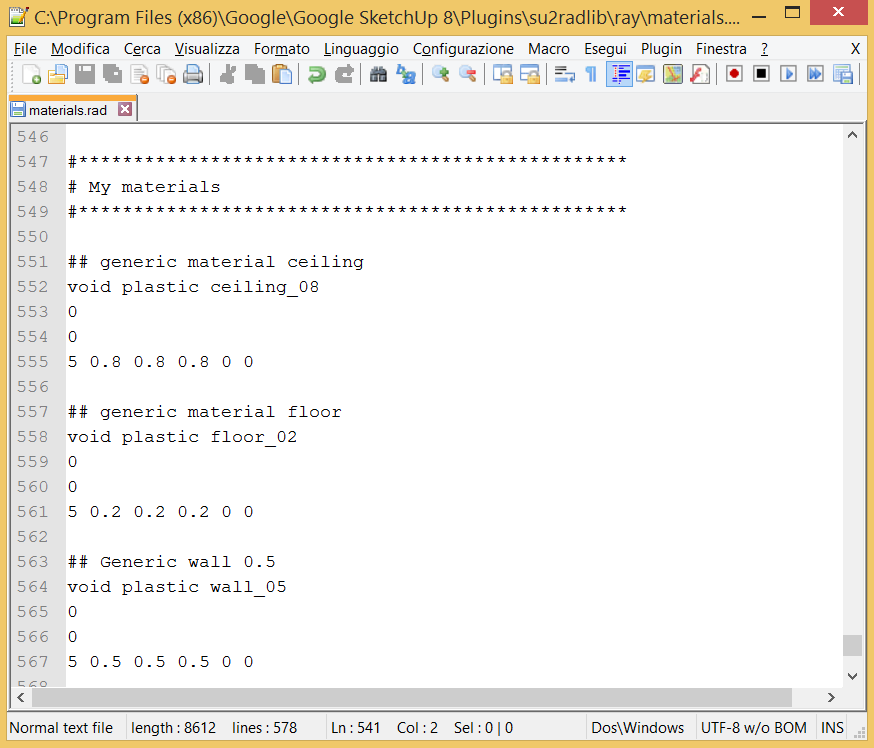
\includegraphics[width=0.7\textwidth]{materialrad}
\caption{\label{img1:materialrad} Definition of custom materials within the su2rad material library}
\end{figure}
Once a material has been added to the library, it became available in SketchUp and can be associate to a layer in the material window in figure \ref{img1:materials}.

\paragraph{Adding material in the material.rad file exported}
If no material is assigned in SketchUp, then SketchUp will assign a default material to each layer. The material.rad file exported by su2rad will appear as in figure \ref{img1:materialexported}. Delete the SketchUp default material and write your materials keeping in mind two important things:
\begin{itemize}
\renewcommand{\labelitemi}{\tiny$\blacksquare$}
\item use the syntax shown at the begin of this section
\item use for the ID of the material the name of the MODIFIER of the object (in this case the name of the layer, e.g. ceiling, floor, etc.) to combine material and geometry, as shown in figure \ref{img1:combine}
\end{itemize} 
Once created the material for each layer and wrote them in to the materials.rad file it will seem like in Figure \ref{img1:materialmodif}.
\begin{figure}[h]
\centering
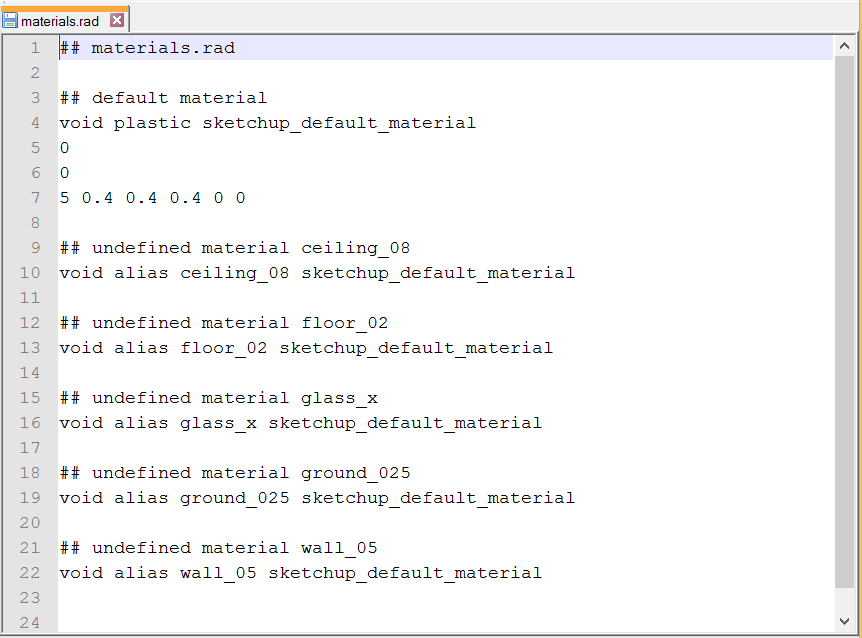
\includegraphics[width=0.7\textwidth]{materialexported}
\caption{\label{img1:materialexported} material.rad exported with default SkectchUp materials}
\end{figure}


\begin{figure}[h]
\centering
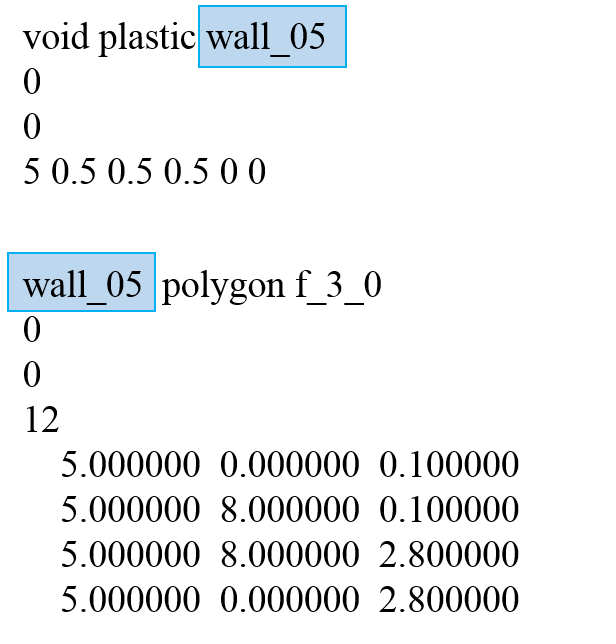
\includegraphics[width=0.4\textwidth]{combine}
\caption{\label{img1:combine} Combine the material and the geometry using the MODIFIER of the object as ID of the material}
\end{figure}

\begin{figure}[h]
\centering
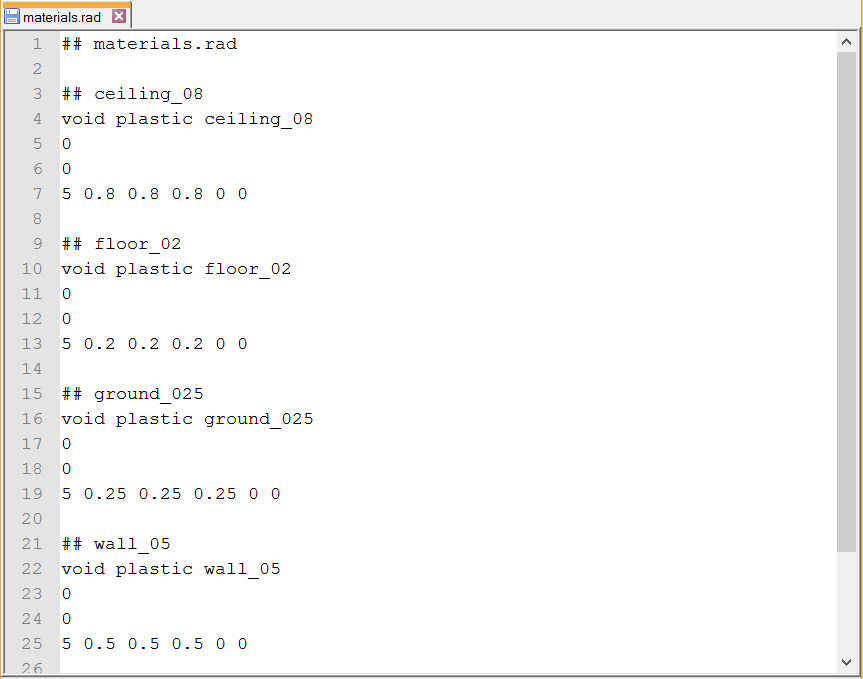
\includegraphics[width=0.7\textwidth]{materialmodif}
\caption{\label{img1:materialmodif} materials.rad with the materials defined by the user}
\end{figure}




\chapter{Creating the CFS model}\label{sec:cfs}
The BSDF data can be generate through several methods: window modelling software (e.g. WINDOW 7.3), simulation programs (e.g. TrancePro or Radiance's "genBSDF") or measurements with a goniophotometer. In this section will be give an overview of the BSDF file creation with the software WINDOW 7.3.\\

We will use the software WINDOW 7.3 by LBNL for the BSDF generation. The tool can be downloaded from \url{http://windows.lbl.gov/software/window/window.html}.
Firstly, adjust the optical calculation options in the software preferences, \textit{File -> Preferences}. Checking the relative boxes as shown in figure \ref{img2:preference}, WINDOW gives in output the BSDF matrices of the complete fenestration system in an xml extension. In particular, it is also possible to have in output the BSDF data for both solar and visible band, remembering that Radiance only uses the front transmission data in the visible range. 
%On the other side, for the thermal simulation it is required also the solar band. 

\begin{figure}[h]
\centering
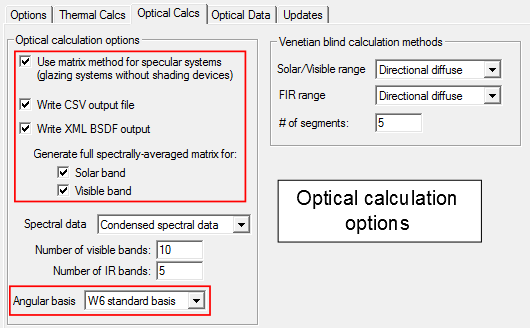
\includegraphics[width=0.7\textwidth]{preference}
\caption{\label{img2:preference} Preference setting in WINDOW 7.3}
\end{figure}

Particular attention should be paid to the angular basis option; this option defines the sky division in order to have a BSDF matrix 145x145 size, and to avoid error in the simulation. It is required to set the "W6 standard basis" (Figure \ref{img2:preference}) that correspond to the Klems division.

Once adjusted the preferences, move to the \textit{Glazing System Library} (figure \ref{img2:windowglass}) where it is possible to create the fenestration system choosing the glass and the shade typology from the respective database (IGDB and CGDB). First, create a double pan-glass low-e as in Figure \ref{img2:windowglass}, name it "2pan\_lowe" and export it following the tutorial \url{http://sel.me.wisc.edu/trnsys/downloads/tutorials_and_examples/window5/windowtutorial.pdf} in order to make available this new system in TRNSYS. Then click the Calc [F9] button in order to create the BSDF file of this system in xml extension.\\


\begin{figure}[h]
\centering
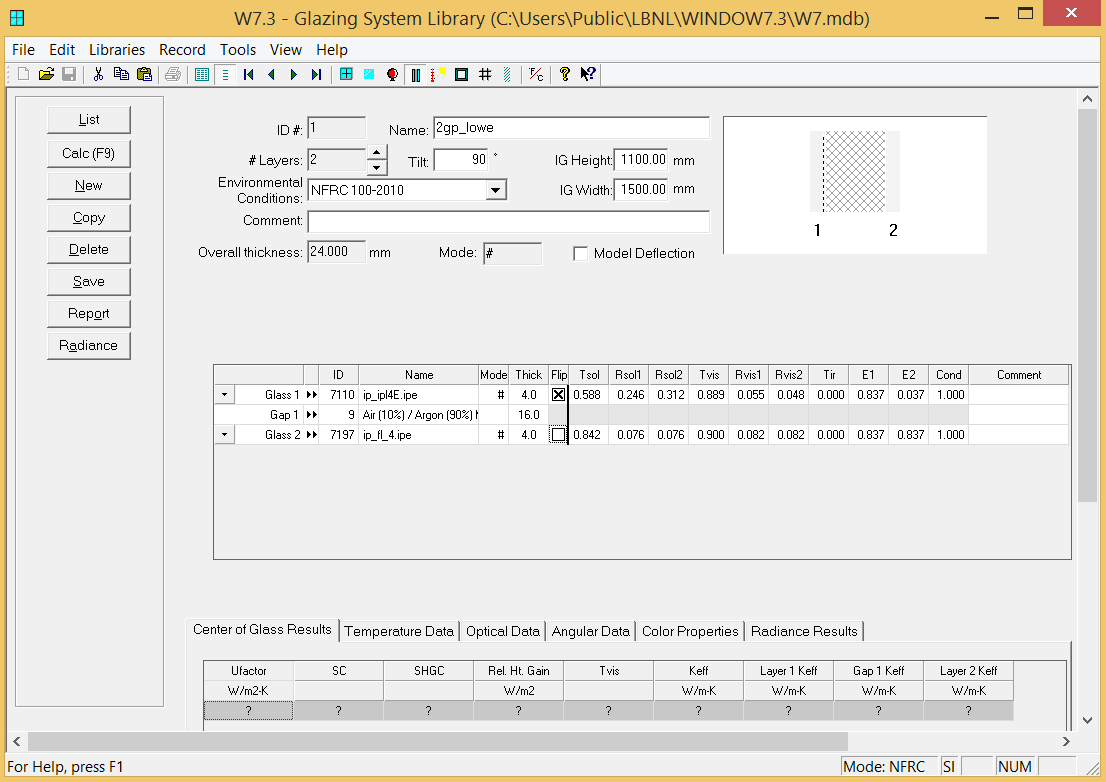
\includegraphics[width=0.9\textwidth]{windowglass}
\caption{\label{img2:windowglass} Base configuration system in Glazing System Library}
\end{figure}

In order to add the shading increase the number of layer to 3 and select "shade or frit" from the drop down list for the first (Figure \ref{img2:window73_2}).
\begin{figure}[h]
\centering
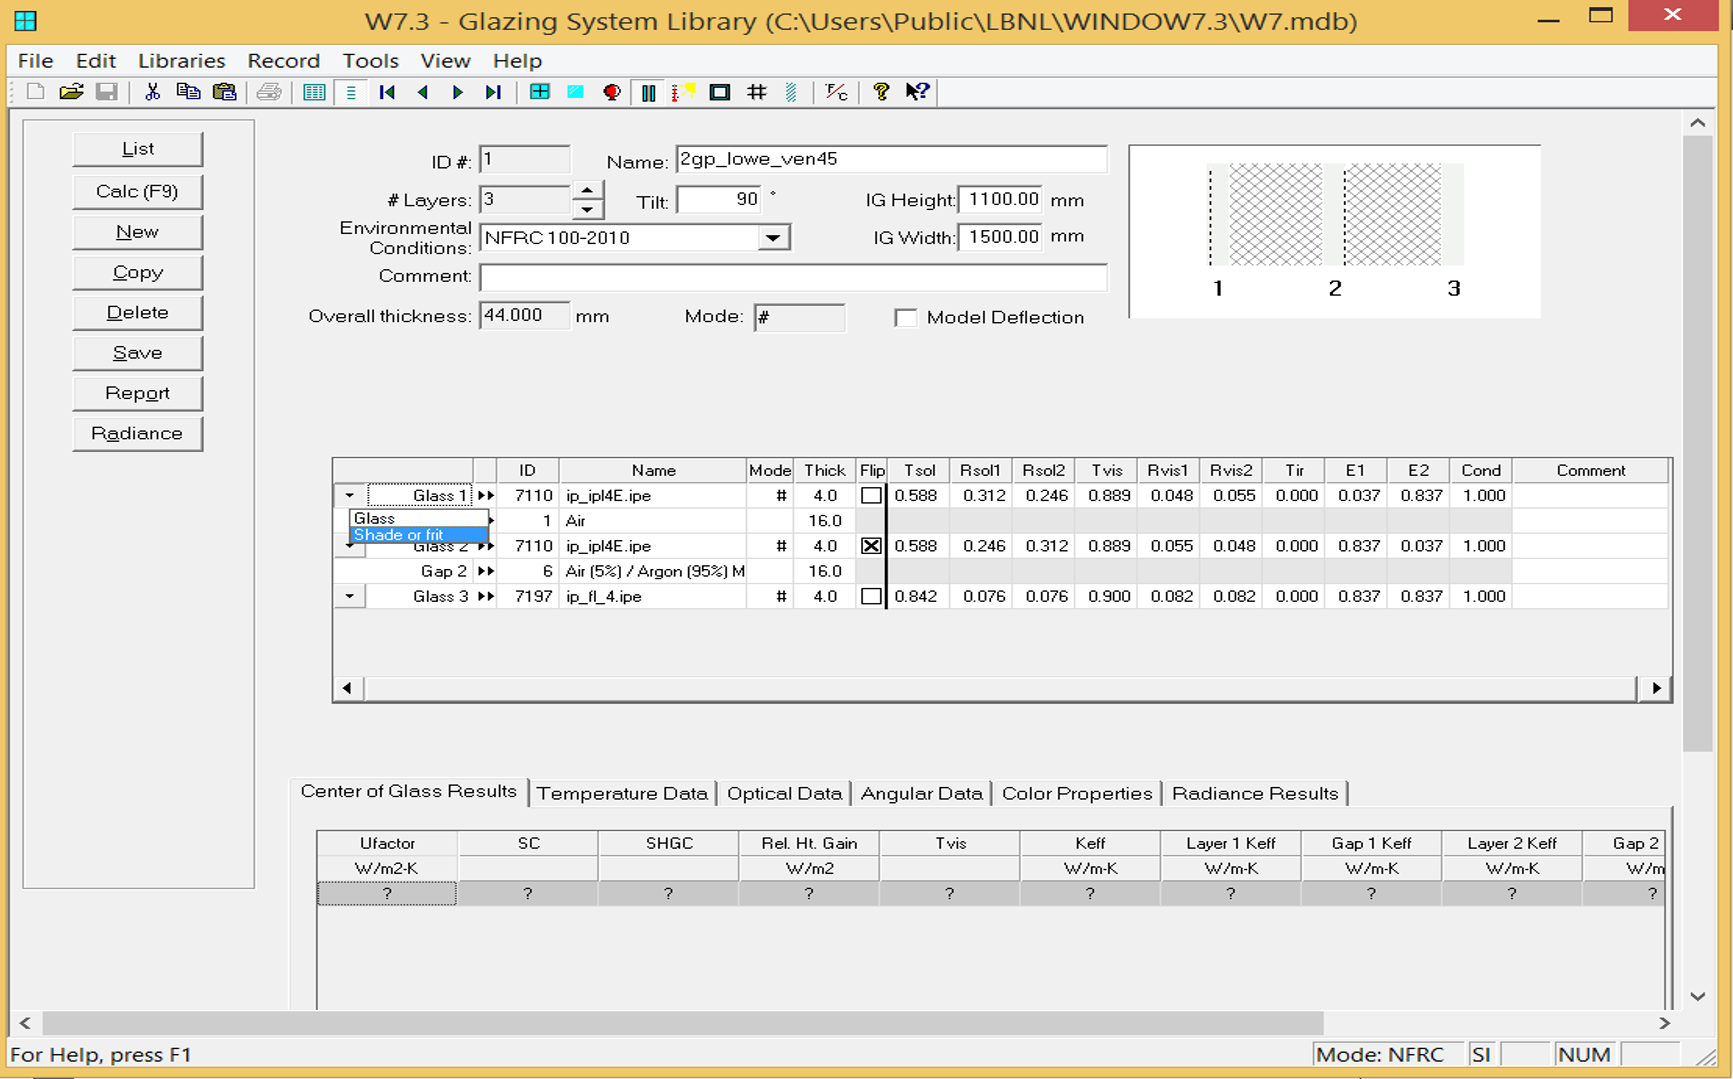
\includegraphics[width=0.9\textwidth]{window73_2}
\caption{\label{img2:window73_2} Adding the shading layer in Glazing System Library}
\end{figure}

In \textit{Shading Layer Library} (Figure \ref{img2:shading}) the shade properties can be adjusted or a new shade can be create, choosing between: venetian blinds, homogeneous diffusing shade, woven shade, fritted shade. Then, for each typology, it is possible to choose geometric and optical parameters. WINDOW allows also to use BSDF data pre-calculated in the shading type by selecting "shade with XML data". 

\begin{figure}[h]
\centering
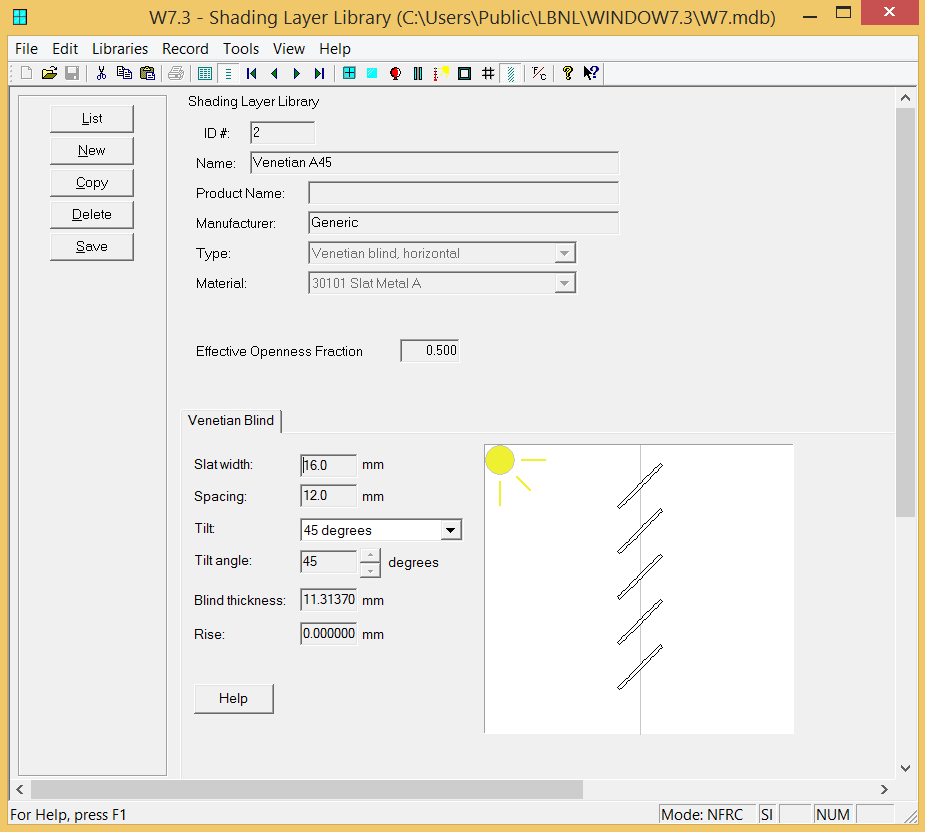
\includegraphics[width=0.9\textwidth]{shading}
\caption{\label{img2:shading} Venetian blinds configuration in Shading Layer Library}
\end{figure}

Select the shading in Figure \ref{img2:shading} for the shading layer and you will obtain a complete system as in Figure \ref{img2:window73} and name it with a name easy to recognize (e.g. 2pan\_lowe\_venetian45).

\begin{figure}[h]
\centering
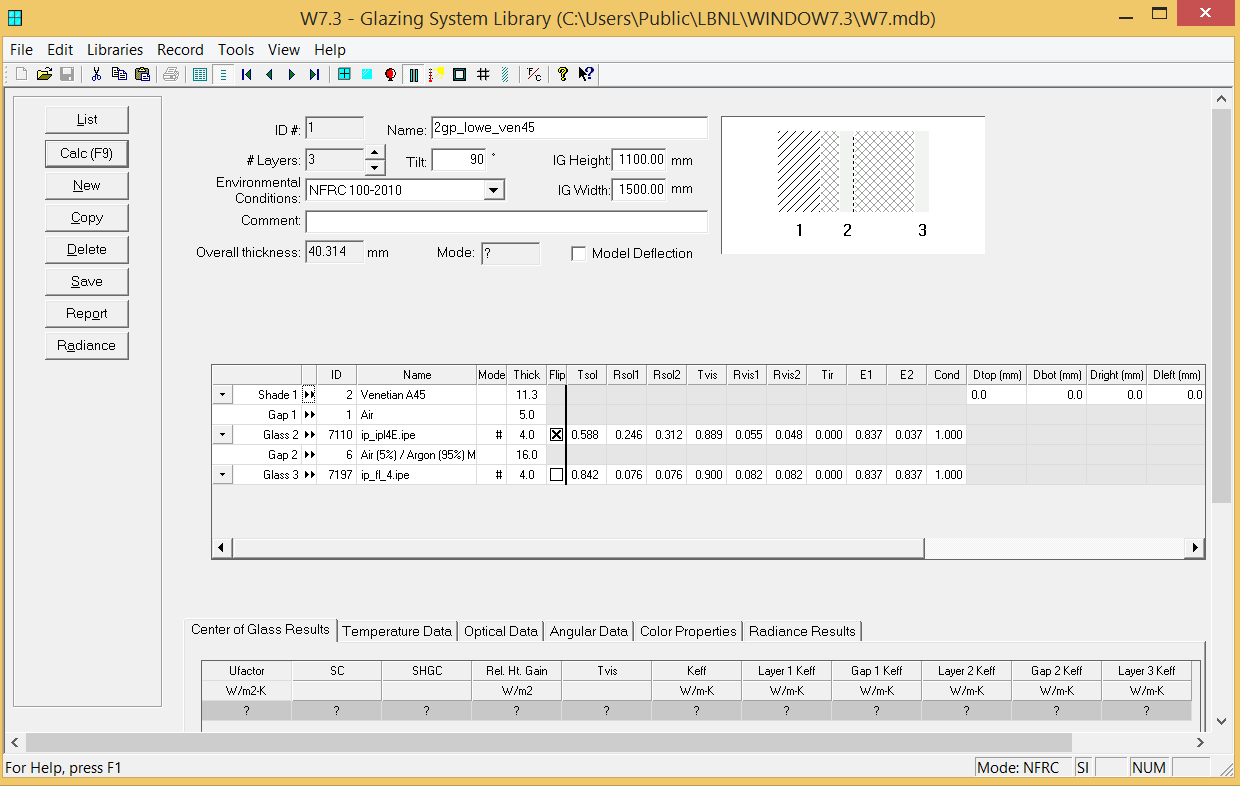
\includegraphics[width=0.9\textwidth]{window73}
\caption{\label{img2:window73} Complete glazing system in Glazing System Library}
\end{figure}

Click again the \textit{Calc} [F9] button. An xml file with the name of the system will be created in the directory
\begin{center}
\textit{C:\textbackslash Users\textbackslash Public\textbackslash LBNL\textbackslash WINDOW7.3\textbackslash BSDFs}
\end{center}

Create, with the same steps above, the BSDFs file for the configuration with blinds at 0 and 90-degree tilt angle in order to define a dynamic shading system.\\
Rename the BSDF file with a integer number starting with the number 0 that correspond to the base configuration (e.g. glass without shading) and increase the numeration starting from the more open configuration (0-degree tilt angle) to the more closer (90-degree tilt angle). \\
The BSDF file created has to be locate it in a specific folder where the TypeDLT can find it (see Chapter \ref{sec:manualtweaks}).\\
\chapter{Manual tweaks} \label{sec:manualtweaks}

First is required to bring the folder create by su2rad in the project folder of the TRNSYS simulation, and rename the folder Zone{\color{red} N} where {\color{red} N} is a positive integer number that define the zone analysed.\\
In figure \ref{img4:zone1} is shown an example of how locate the folder in the right place. The integer number that identifies the zone is the same number that has to be defined in Type's control panel under the input \textit{ZoneID}.
\begin{figure}[h]
\centering
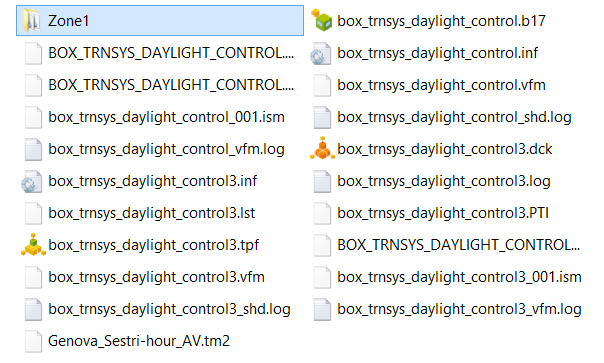
\includegraphics[width=0.7\textwidth]{zone1}
\caption{\label{img4:zone1} Positioning of the Radiance simulation folder in the TRNSYS project folder}
\end{figure}

Within the folder Zone1 is then necessary creating some folders: 
\begin{itemize}
\renewcommand{\labelitemi}{\tiny$\blacksquare$}
\item {\color{blue} data}, it will contain the matrices for the calculation, the file with the sensors grid and another subfolder:
\subitem{\tiny$\blacksquare$} {\color{blue} bsdf}, it will contain the bsdf data listed with integer numbers
\item {\color{blue} temp}, it will contain temporary files create during the matrices generation
\item {\color{blue} window}, it will contain the windows in the scene and a new file called win.vd
\end{itemize}

And deleting some other unused folder:
\begin{itemize}
\renewcommand{\labelitemi}{\tiny$\blacksquare$}
\item ambfiles
\item images
\item logfiles
\item octrees
\item skies
\end{itemize}

In order to make available the input data for TypeDLT it is necessary to modify some files generated by SketchUp and to create a new one, which will collect all the windows in the scene. Use a simple text editor to make these changes.\\
The 3PM requires that the windows in the scene are a secondary light source, so that the user has to change the windows material in glow material, see three-phase method tutorial for in-depth analysis. To do this the user has to open the rad file containing the window/windows geometries and add in the heading of this file the glow material definition paying attention to correspond the modifier of the geometry with the ID of the glow material as shown in figure \ref{img4:winglow}. Figure \ref{img4:wingroup} shows the case of a group windows. Then, move the window\_south.rad file from the "objects" folders to the "window" folder.

\begin{figure}[h] 
\centering
  \subfigure[]{% 
    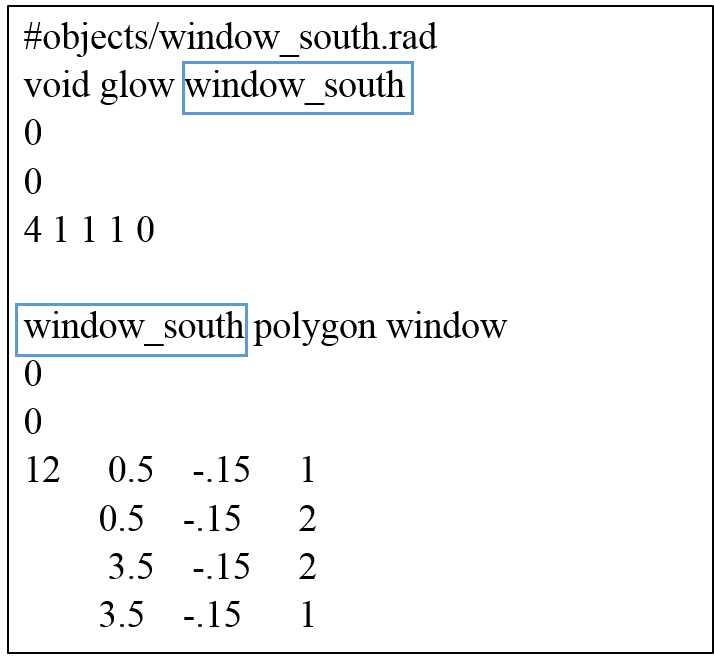
\includegraphics[width=.35\textwidth]{win} \label{img4:win} 
  }
  \subfigure[]{% 
    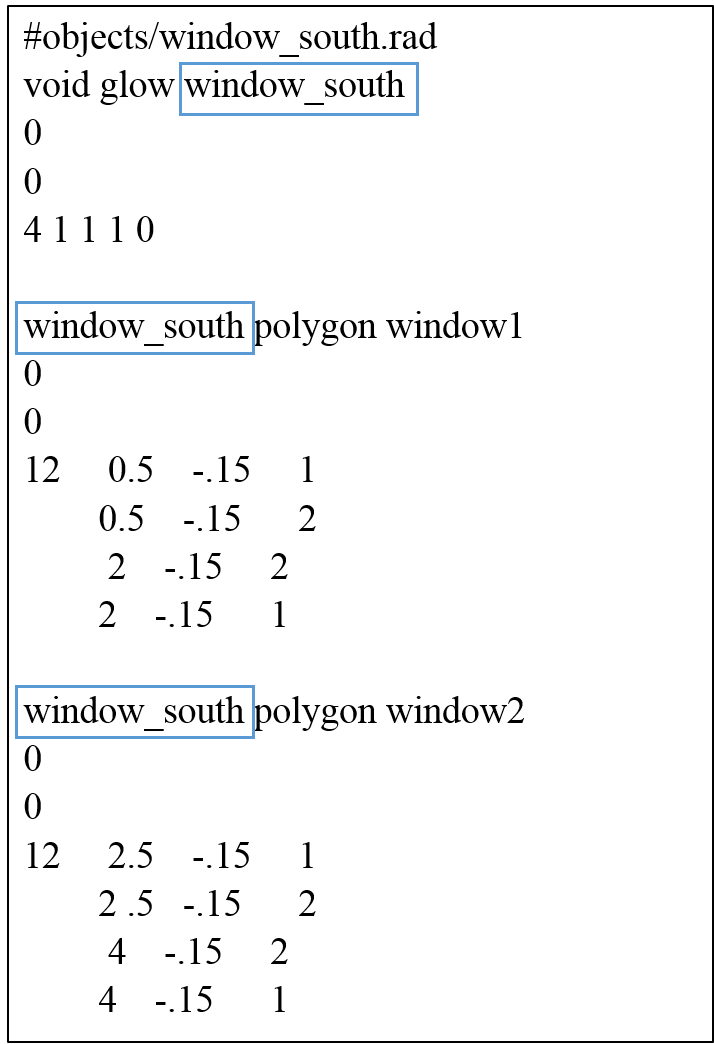
\includegraphics[width=.35\textwidth]{wingroup} \label{img4:wingroup} 
  } 
  \caption{\label{img4:winglow} Window file modified with the glow material for one window \ref{img4:win} and a group of two windows \ref{img4:wingroup}}
\end{figure}

A new file called {\color{blue} win.vd} has to be created within the "window" folder. In this new file insert the number of windows/group of windows and the  list of this windows/group of windows following a specific format: window modifier, view direction (vd) and view up (vp). The view direction is the window normal vector facing toward the outside of the room, the view up is the window up vector, vd and vu are always orthogonal. Figure \ref{img4:windoworient} shows how to choose vd and vu from a sample geometry in which there is a window facing south. It is also shown how to report these information in the win.vd file for a window with modifier window\_south.

\begin{figure}[H]
\centering
\begin{minipage}[c]{0.6\linewidth}
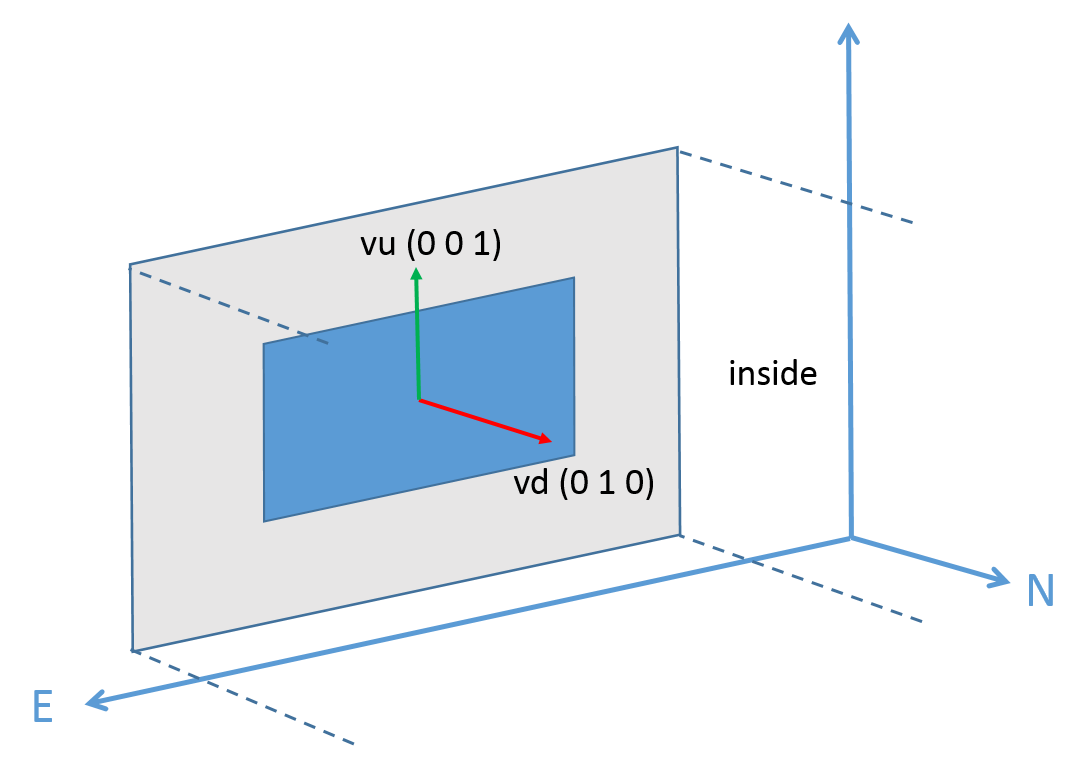
\includegraphics[width=1\textwidth]{windraw}
\end{minipage}
\quad
\begin{minipage}[c]{0.3\linewidth}
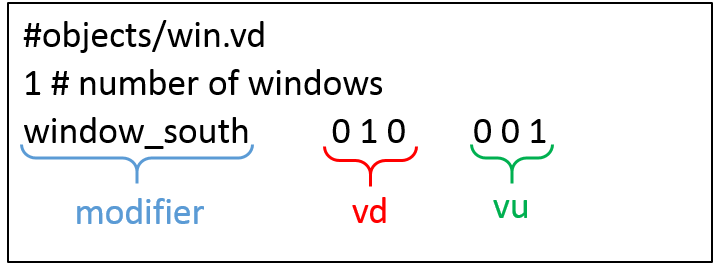
\includegraphics[width=1\textwidth]{winvd}
\end{minipage}
\caption{\label{img4:windoworient} New file with the list of windows in the scene and orientation of the vu and vd vectors}
\end{figure}

At the end you will have two files in the "window" folder, the win.vd and the window\_south.rad. Pay attention that the name \underline{window\_south} has to be the same for:
\begin{itemize}
\item *.rad file
\item window modifier within the *.rad file
\item window modifier within the win.vd file
\end{itemize}
as shown by the red rectangle in Figure \ref{img4:window_name}.

\begin{figure}[h]
\centering
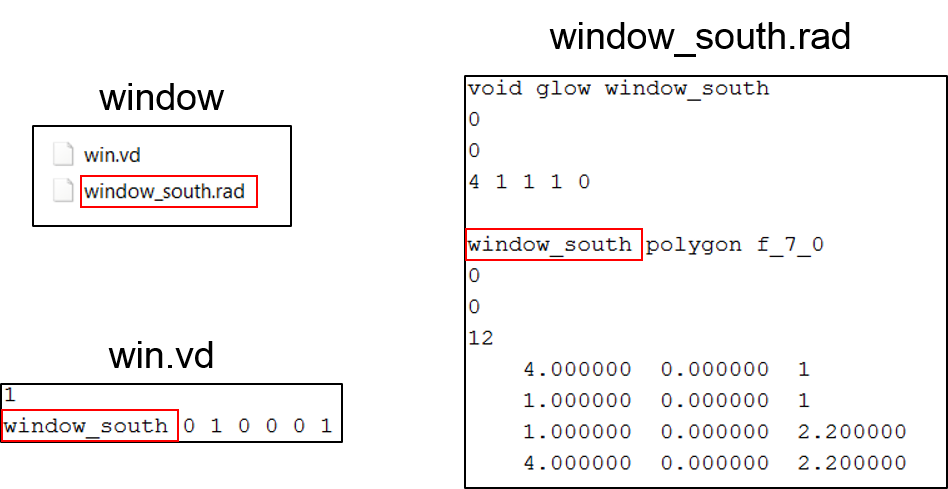
\includegraphics[width=0.7\textwidth]{window_name}
\caption{\label{img4:window_name} Correspondence on the window name within the several files}
\end{figure}

Delete some rows from the rad file that contains all the objects into the scene, Zone1.rad in this case (Figure \ref{img4:tutorial2}). In particular, the row that calls the sky definition and the window objects. In fact, TypeDLT creates at each time step a new sky file with the information contained in the weather file. And, the window/group of windows are used only for the matrices generations, during the simulations will be used the BSDFs data.

\begin{figure}[h]
\centering
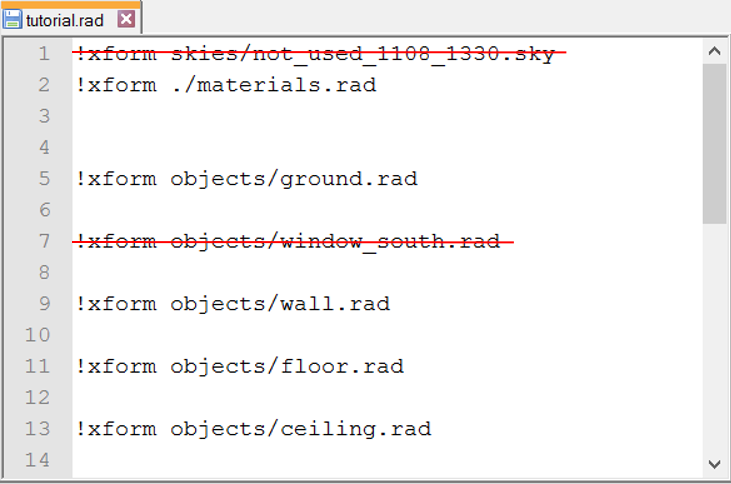
\includegraphics[width=0.6\textwidth]{tutorial2}
\caption{\label{img4:tutorial2} Contents of the tutorial.rad file}
\end{figure}

Finally, add the file containing the sensors grid within the \textit{data} folder with the the specific name {\color{blue}grid.pts}. The format to follow is: x, y, z, dx, dy, dz where x, y and z are the three dimensional coordinates of the point and dx,dy and dz are the coordinates of the vector that define view direction of the sensor.
The example file (figure \ref{img4:grid}) is composed by row grid with 9 sensors located in the middle of the scene 1 meter from the window with a step of 0.5 m.

\begin{figure}[h]
\centering
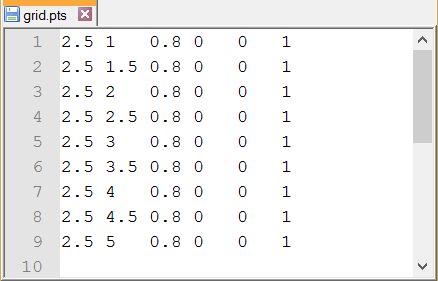
\includegraphics[width=0.5\textwidth]{grid}
\caption{\label{img4:grid} Format of the file containing the sensors grid}
\end{figure}

\section{Checking of the surface normal direction} \label{sec:normalsurf}

Before starting the simulations it is necessary to verify the right orientation of the window towards the inside of the room.
To do this follow this procedure: 
\begin{enumerate}
\item Open the command prompt of Windows following the steps:
\begin{itemize}
\item Type WinKey + R
\item Input "cmd"
\item Type Enter
\end{itemize}
\item Move into the Zone1 folder within the command prompt. Type "cd" (change directory) followed by the path of the Zone1 folder  in the command line 
\begin{center}
cd path\textbackslash of\textbackslash folder\textbackslash Zone1
\end{center}

\item Create a binary file containing the whole scene writing in the terminal the command 
\begin{center}
oconv materials.rad Zone1.rad window\textbackslash window\_south.rad > temp\textbackslash model.oct
\end{center}
this command converts the text format file of the scene in a binary format file readable by the Radiance functions. Change the name of the window rad files according to your model. Radiance requires to list the materials.rad files always before the geometry (Zone1.rad) it modifies, in your next simulations please follow this sequence in order to avoid errors during this initial step.

\item  Last step, create a preview of the room and check that the surface normal faces the correct direction with the command 
\begin{center}
rvu -ab 2 -vf views\textbackslash south\_view.vf -av 0.2 0.2 0.2 temp\textbackslash model.oct
\end{center}
where ab (ambient bounce) identifies the number of light reflections within the scene; av (ambient value) is used to set the overall light level in the scene, using a value of 0.2 (the three values regard the channels RGB) gives the possibility to see the inside of room even though the surface normal face the incorrect direction (figure \ref{img4:rvublack}). 
\end{enumerate}

If the surface is correctly oriented we will see a white light emitted from the window polygon (figure \ref{img4:rvu}), otherwise we will look at a black room (figure \ref{img4:rvublack}). This because the light material glow emits light only in the direction of the surface normal. \\
In the second case, black room, will be necessary reverse the surface normal. It can be done in SketchUp dropping the cursor on the surface to be reversed, right click on the surface and select \textit{Reverse Faces}. At this point export the window, with the procedure explained in section \ref{sec:export}, replace it with the incorrect one and run again the test.


\begin{figure}[h] 
\centering
  \subfigure[Surface normal correct direction]{% 
    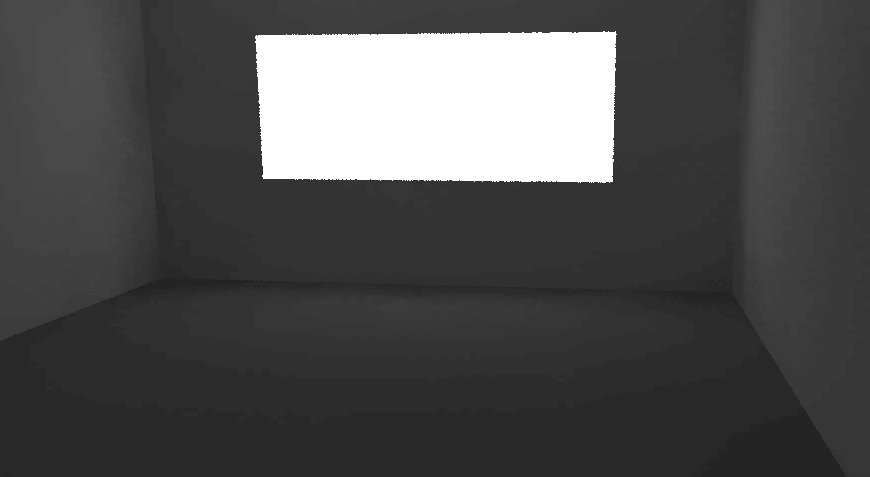
\includegraphics[width=.7\textwidth]{rvu} \label{img4:rvu} 
  } 
  \subfigure[Surface normal incorrect direction]{% 
    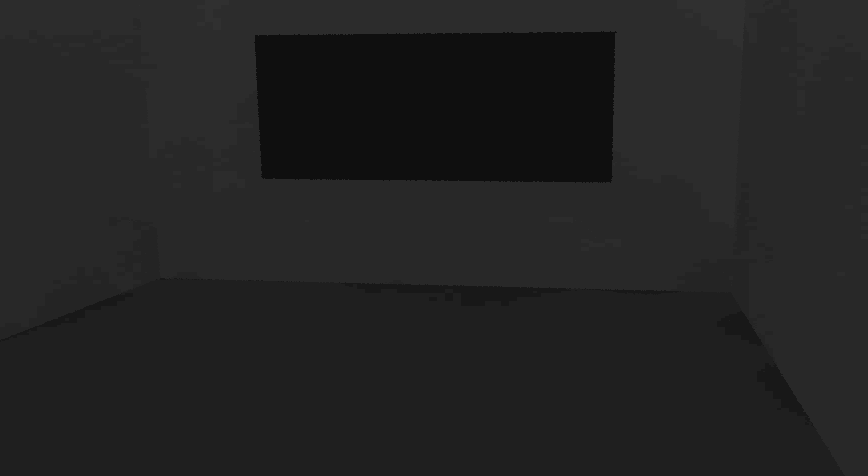
\includegraphics[width=.7\textwidth]{rvublack} \label{img4:rvublack} 
  }
  \caption{\label{img4:surfacenormal} rvu rendering of the inside room without and with light emitting window polygon }
\end{figure}
 





\chapter{Implementation in TRNSYS}

The last chapter regard the implementation in TRNSYS. At this point, remain to define the thermal model that can be done following the tutorial of TRNSYS3D plug-in for SketchUp in the TRNSYS documentation folder:
\begin{center}
....\textbackslash Trnsys17\textbackslash Documentation\textbackslash A4\_3DBuildingTutorial.pdf
\end{center} 
However, skip the preparation of the thermal model and use the TRNSYS deck (tutorial\_imported.tpf) provided within the file example. The TRNSYS deck has been created from one of the default project suggested by TRNSYS when a new project is selected. To this default deck four new elements have been added, the TypeDLT and three equations, to reach the configuration in  Figure \ref{img5:deck}. 
\begin{figure}[H]
\centering
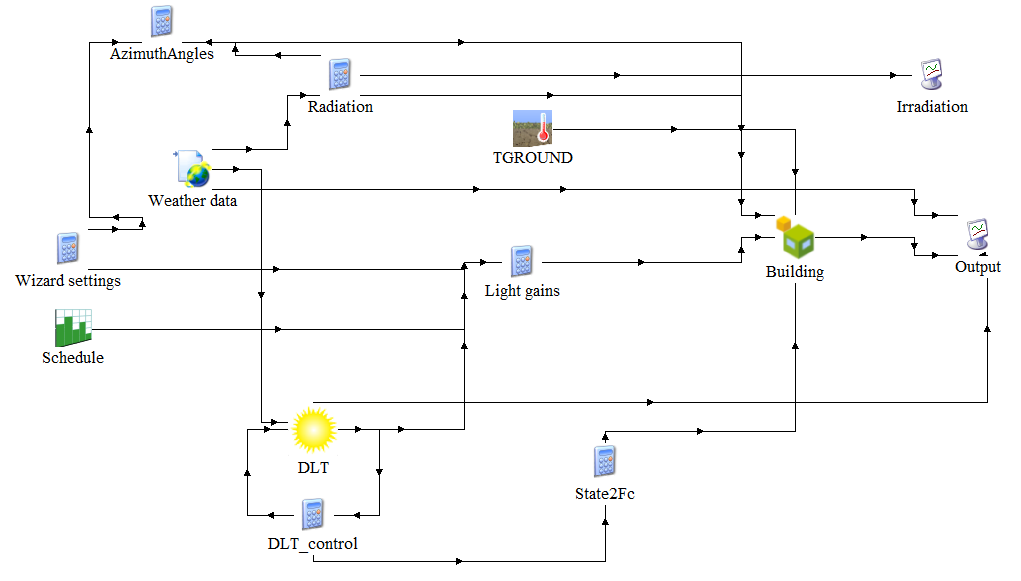
\includegraphics[width=1\textwidth]{deck}
\caption{\label{img5:deck} TRNSYS deck with the TypeDLT}
\end{figure}
One equation is used to define the control algorithm (DLT\_control), one is used to calculate the external gain due to artificial light (Light gains) of dimmed system and is direct connected to the Type56, the last equation is used to convert the shading state chose by the control in a shading factor-Fc (State2Fc) value that is passed to the Type56 and reduce of a certain percentage the transparent area of the window.\\
Copy and paste the "Zone1" folder containing the daylighting model within the project folder as specified in the Chapter \ref{sec:manualtweaks}. If you are not sure of the correct ending of the previous steps please compare your Zone1 folder with the one provided. \\
In the deck provided the input data have been already connected. Please note that from the "Weather data" Type are connected:
\begin{itemize}
\renewcommand{\labelitemi}{\tiny$\blacksquare$}
\item Latitude and Longitude 
\item Direct normal and diffuse horizontal illuminance
\item Month, day of the month and hour of the day
\end{itemize}  
Double clicking on the TypeDLT icon, observe that the Zone ID is set on 1 corresponding to name of the folder "Zone1". In addition, the Control is connected with the Equation Type "DLT\_control".\\
In Chapter \ref{sec:cfs} four files BSDF have been create. In particular, the file 0.xml correspond to the base configuration without shadings, the 1.xml, 2.xml and 3.xml correspond respectively to the configurations with shading tilted at 0, 45 and 90 degree angle.

\begin{figure}[h]
\centering
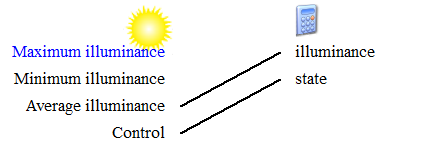
\includegraphics[width=0.6\textwidth]{controlinput}
\caption{\label{img5:controlinput} Input control equation}
\end{figure}

The control strategy of this system is based on the daylight availability within the zone and takes in input two parameters: average illuminance and control (current shading state), see Figure \ref{img5:controlinput}. The aim is to find the shading state that provide an internal illuminance within the range 300-3000 lux. The state does not change if the threshold limits are already respected.\\
The "State2Fc" equation takes in input the current shading state and gives in output a Fc value that represent the percentage of opaque area due to the shading respect to the glazing surface. Then, the Fc is passed to the Type56 as external shading factor (Figure \ref{img5:windowtrnsys}). Notice also that the glazing system created in WINDOW7.3 has been imported in TRNSYS and used in the simulation. \\
For the conversion of shading state into shading factor the energy balance in the equation \ref{eq:fc} has been used.

\begin{equation}\label{eq:fc}
Fc = 1 - \dfrac{SHGC \tb{glass+shading}}{SHGC \tb{glass}}
\end{equation}

where SHGC \tb{shading+glass} and SHGC \tb{glass} are the Solar Heat Gain Coefficients respectively of the whole systems, glazing and shading, and of the glazing system only. Both these values are calculated by WINDOW 7.3. 

\begin{figure}[h]
\centering
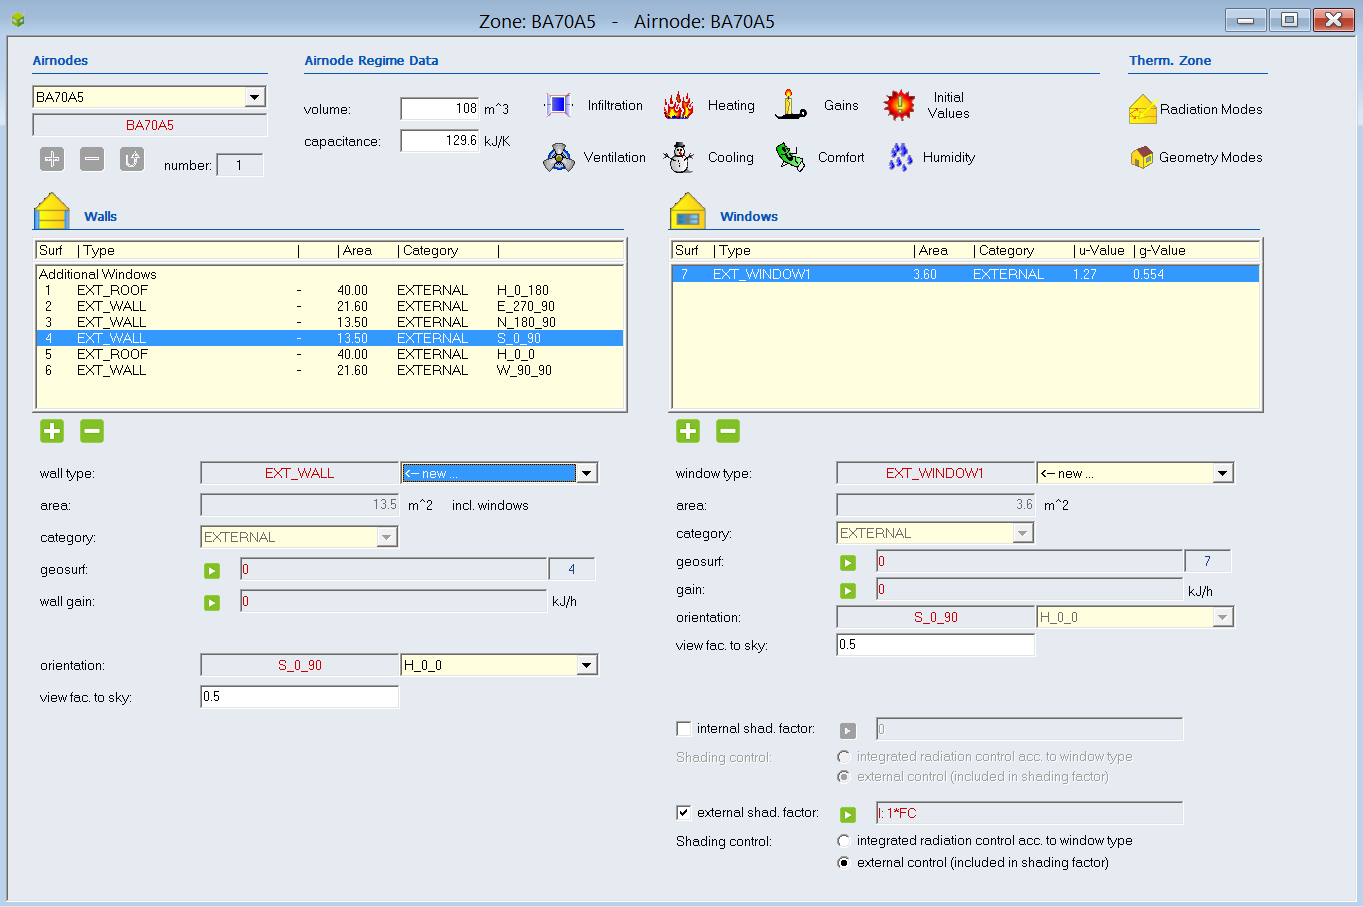
\includegraphics[width=0.7\textwidth]{windowtrnsys}
\caption{\label{img5:windowtrnsys} Zone window - Fc input as external shading factor}
\end{figure}

\begin{figure}[H]
\centering
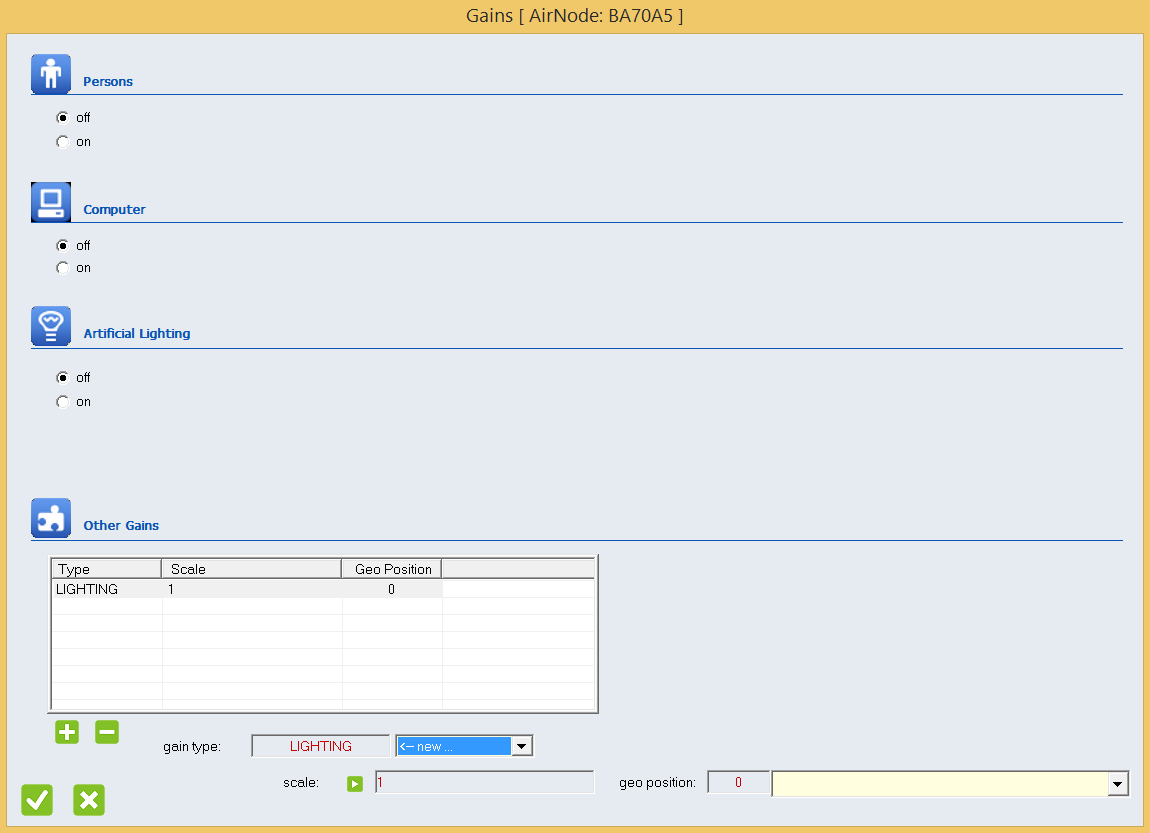
\includegraphics[width=0.7\textwidth]{gain}
\caption{\label{img5:gain} Gain window - The Artificial lighting gain is considered as Other gain from the TRNSYS deck}
\end{figure}

The gains due to the artificial lighting are calculated through an ad hoc equation. The equation "Light gains" takes in input the minimum illuminance level over the sensors grid from the TypeDLT and if the natural light is lower than the threshold value of 500 lux the artificial light is dimmed to reach this level. The artificial light power required to arrive at 500 lux is converted in heat gain and passed at each time step to the Type56 as external gain (Figure \ref{img5:gain}). \\
Once explained how the deck works let's simulate. Click \textit{Calculate -> Run simulation [F8]}, first the view and daylighting matrices will be calculate (Figure \ref{img5:matrices}). The matrices generation requires several  minutes depending also by the complexity of the geometry.

\begin{figure}[h] 
\centering
  \subfigure[View matrix generation]{% 
    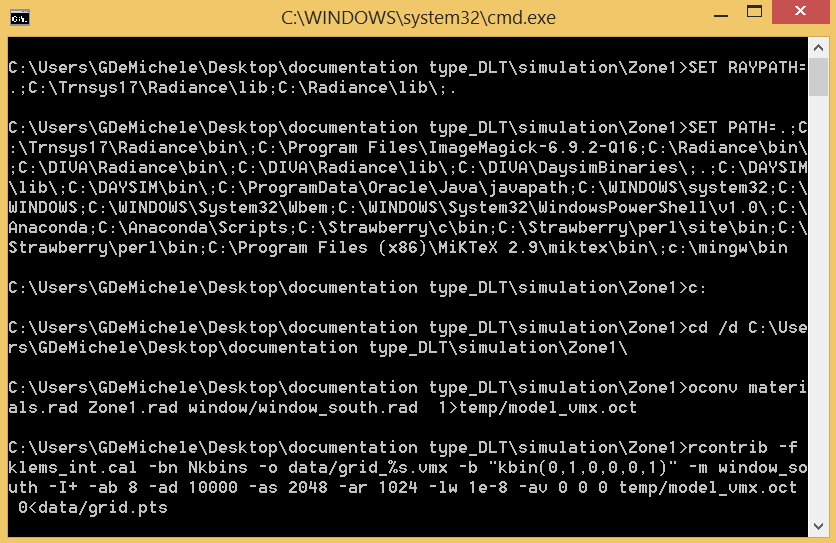
\includegraphics[width=.45\textwidth]{vmx} \label{img5:vmx} 
  } 
  \subfigure[Daylighting matrix generation]{% 
    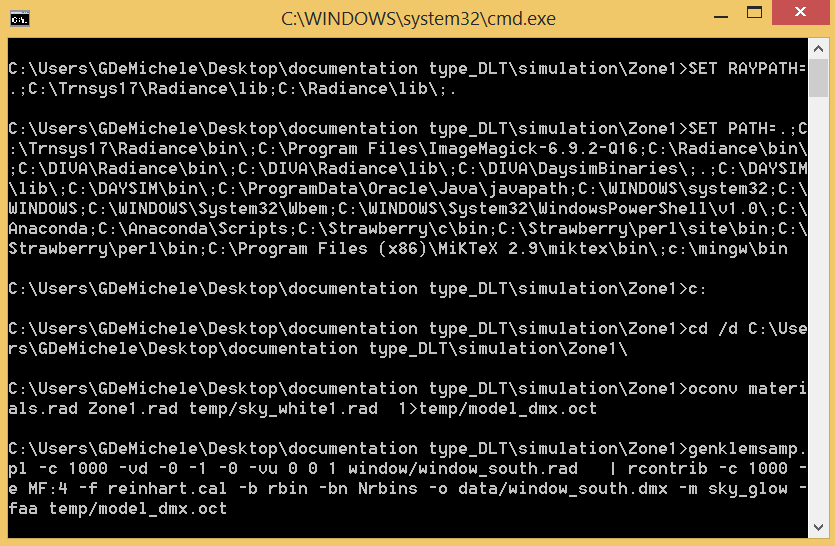
\includegraphics[width=.45\textwidth]{dmx} \label{img5:dmx} 
  }
  \caption{\label{img5:matrices} View and daylighting matrix generation}
\end{figure}

At each time-step will be created the sky vector and performed the matrices multiplication (Figure \ref{img5:3pm}) that require few seconds. Within the time step the control decides if change state and run another daylighting simulation or go ahead with the thermal simulation and the next time step.

\begin{figure}[h]
\centering
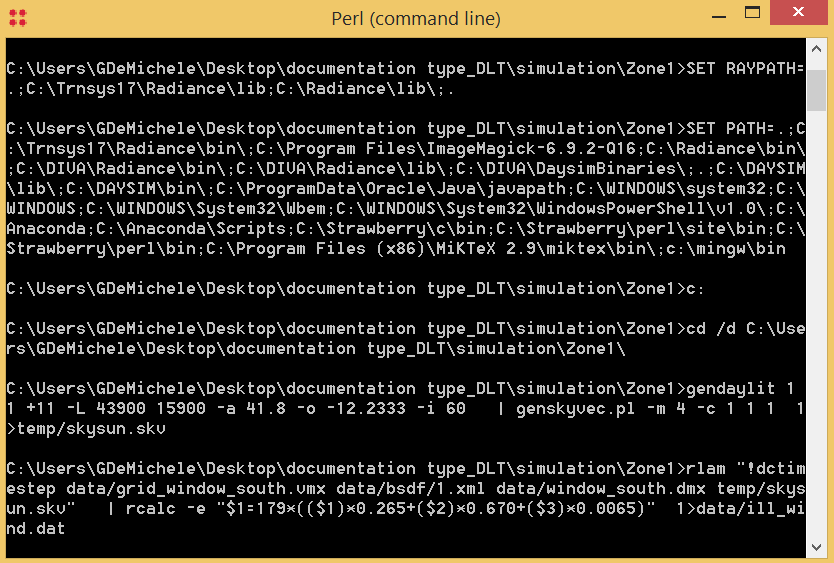
\includegraphics[width=0.5\textwidth]{3pm}
\caption{\label{img5:3pm} Sky vector generation and matrix multiplication }
\end{figure}


%Once the model is ready, create a new project in the Simulation Studio and locate the TypeDLT onto the TRNSYS deck. First, connect the following variable from the \textit{Weather data} Type: 
%\begin{itemize}
%\renewcommand{\labelitemi}{\tiny$\blacksquare$}
%\item Latitude and Longitude 
%\item Direct normal and diffuse horizontal illuminance
%\item Month, day of the month and hour of the day
%\end{itemize} 
%
%\begin{figure}[h]
%\centering
%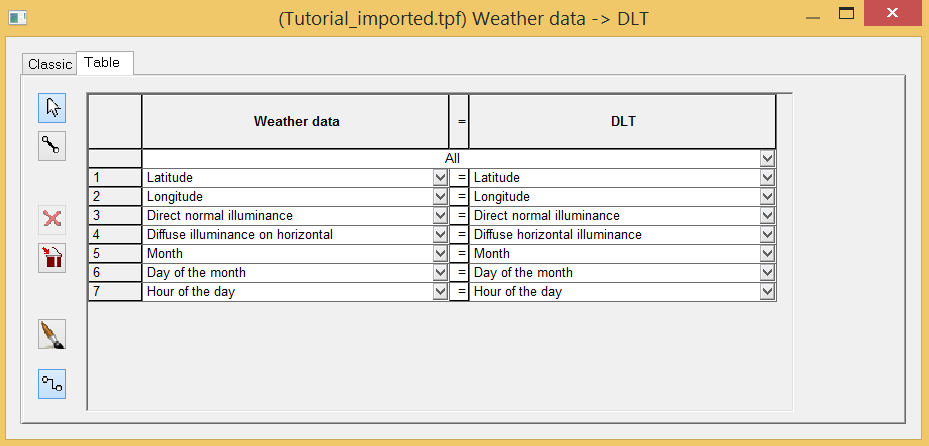
\includegraphics[width=0.7\textwidth]{DLTint}
%\caption{\label{img5:DLTint} Connections between Weather data and TypeDLT}
%\end{figure}
%
%
%Double click on the TypeDLT icon, set within the Type's control panel the Zone ID that correspond to the integer number that you have assigned in the previous section to the folder which contain the Radiance files. The default values is 1 (Figure \ref{img5:DLTinput}).
%
%\begin{figure}[h]
%\centering
%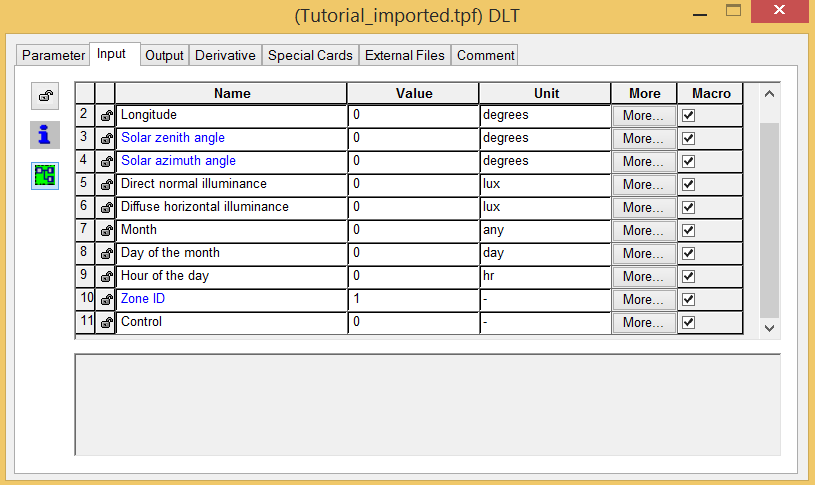
\includegraphics[width=0.7\textwidth]{DLTinput}
%\caption{\label{img5:DLTinput} Input window TypeDLT}
%\end{figure}
%
%At this point, the TypeDLT is ready to simulate and the user can connect the Type's outputs and inputs following its needs.\\
%\begin{figure}[h]
%\centering
%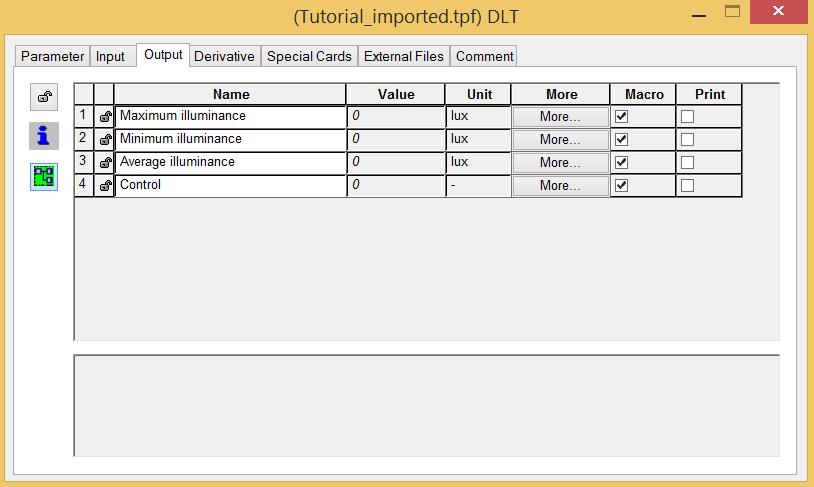
\includegraphics[width=0.7\textwidth]{DLToutput}
%\caption{\label{img5:DLToutput} Output window TypeDLT }
%\end{figure}
%Once the TRNSYS deck is ready and the first simulation is run the view and daylighting matrices (see the manual for the theory) are generated and two terminal windows will be opened, Figure \ref{img5:matrices}.
%
%\begin{figure}[h] 
%\centering
%  \subfigure[View matrix generation]{% 
%    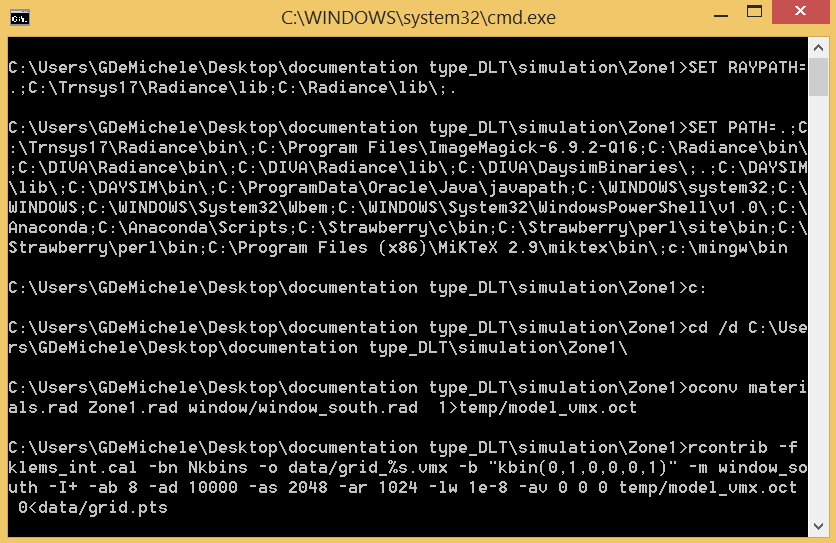
\includegraphics[width=.45\textwidth]{vmx} \label{img5:vmx} 
%  } 
%  \subfigure[Daylighting matrix generation]{% 
%    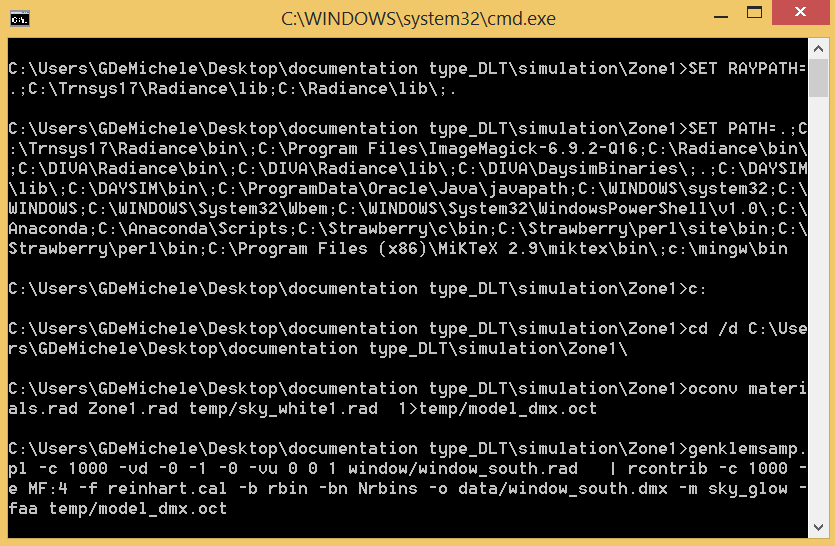
\includegraphics[width=.45\textwidth]{dmx} \label{img5:dmx} 
%  }
%  \caption{\label{img5:matrices} Terminals opened for the view and daylighting matrix generation}
%\end{figure}
%
%The matrices generation requires several  minutes depending also by the complexity of the geometry. Once the matrices are crated it is not necessary to regenerate them for each time-step and for next simulations of the same Radiance scene. At each time-step will be created the sky vector and performed the matrices multiplication (Figure \ref{img5:3pm}) that require few seconds.
%
%\begin{figure}[h]
%\centering
%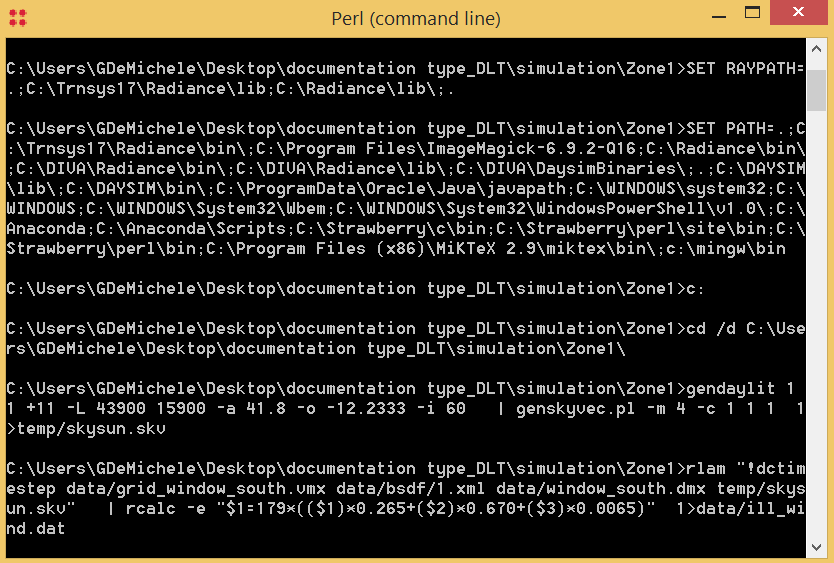
\includegraphics[width=0.5\textwidth]{3pm}
%\caption{\label{img5:3pm} Terminal window - Sky vector generation and matrix multiplication }
%\end{figure}
%
%It is very important to know that the *.vmx and *.dmx file generated are not overwrite in any case, therefore if you need to regenerate these files delete them manually in the folder \textit{data}.\\
%In the following section the example file provided is used to show some of the functionalities offered by the TypeDLT.



%\section{File Example}
%In the example will be shown how to use the outputs for the control of a dynamic shading system and for the calculation of the heat gain due to artificial light. The TRNSYS deck has been created from one of the default project suggested by TRNSYS when a new project is selected. To this default deck four new elements have been added, the TypeDLT and three equations, to reach the configuration in  Figure \ref{img5:deck}. One equation is used to define the control algorithm (\textit{DLT\_control}), one is used to calculate the external gain due to artificial light (\textit{Light gains}) of dimmed system and is direct connected to the Type56, the last equation is used to convert the shading state chose by the control in a shading factor-Fc (\textit{State2Fc}) value that is passed to the Type56 and reduce of a certain percentage the transparent area of the window.
%
%\begin{figure}[H]
%\centering
%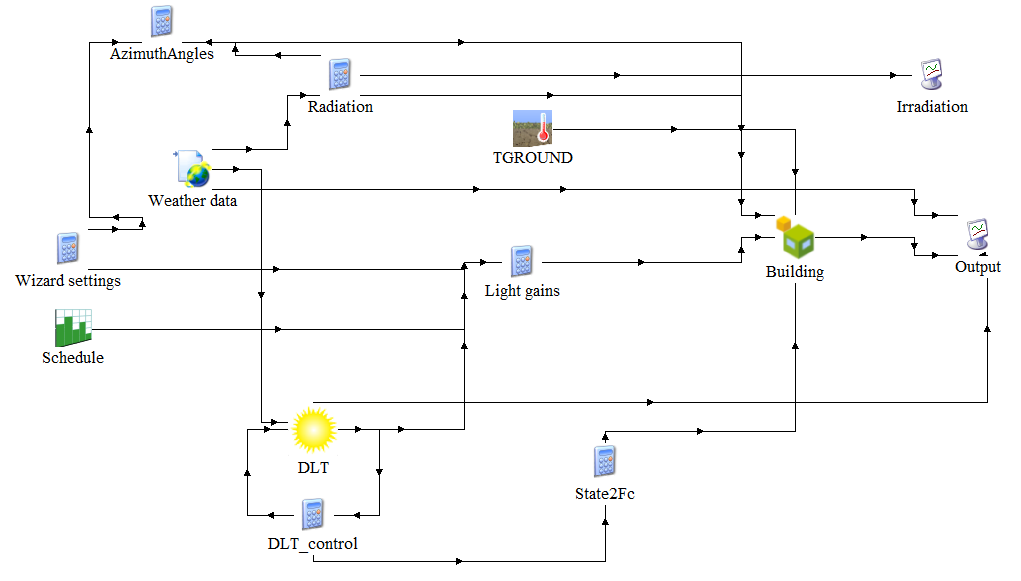
\includegraphics[width=1\textwidth]{deck}
%\caption{\label{img5:deck} TRNSYS deck with the TypeDLT}
%\end{figure}
%
%A dynamic shading systems with external flat lamellas has been considered. Four file BSDF are supplied, the file 0.xml correspond to the configuration without shadings. The 1.xml, 2.xml and 3.xml correspond respectively to the configurations with shading tilted at 0, 45 and 90 degree angle.
%
%
%\begin{figure}[h]
%\centering
%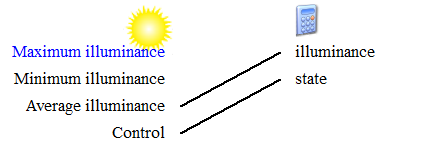
\includegraphics[width=0.6\textwidth]{controlinput}
%\caption{\label{img5:controlinput} Input control equation}
%\end{figure}
%
%The control strategy of this system is based on the daylight availability within the zone and takes in input two parameters: average illuminance and control (current shading state), see Figure \ref{img5:controlinput}. The aim is to find the shading state that provide an internal illuminance within the range 300-3000 lux. The state does not change if the threshold limits are already respected.
%
%The \textit{State2Fc} equation takes in input the current shading state and gives in output a Fc value that represent the percentage of opaque area due to the shading respect to the glazing surface. Then, the Fc is passed to the Type56 as external shading factor (Figure \ref{img5:windowtrnsys}). Notice also that the glazing system created in WINDOW7.3 has been imported in TRNSYS and used in the simulation. \\
%For the conversion of shading state into shading factor the energy balance in the equation \ref{eq:fc} has been used.
%
%\begin{equation}\label{eq:fc}
%Fc = 1 - \dfrac{SHGC \tb{glass+shading}}{SHGC \tb{glass}}
%\end{equation}
%
%where SHGC \tb{shading+glass} and SHGC \tb{glass} are the Solar Heat Gain Coefficients respectively of the whole systems, glazing and shading, and of the glazing system only. Both these values are calculated by WINDOW 7.3. 
%
%\begin{figure}[h]
%\centering
%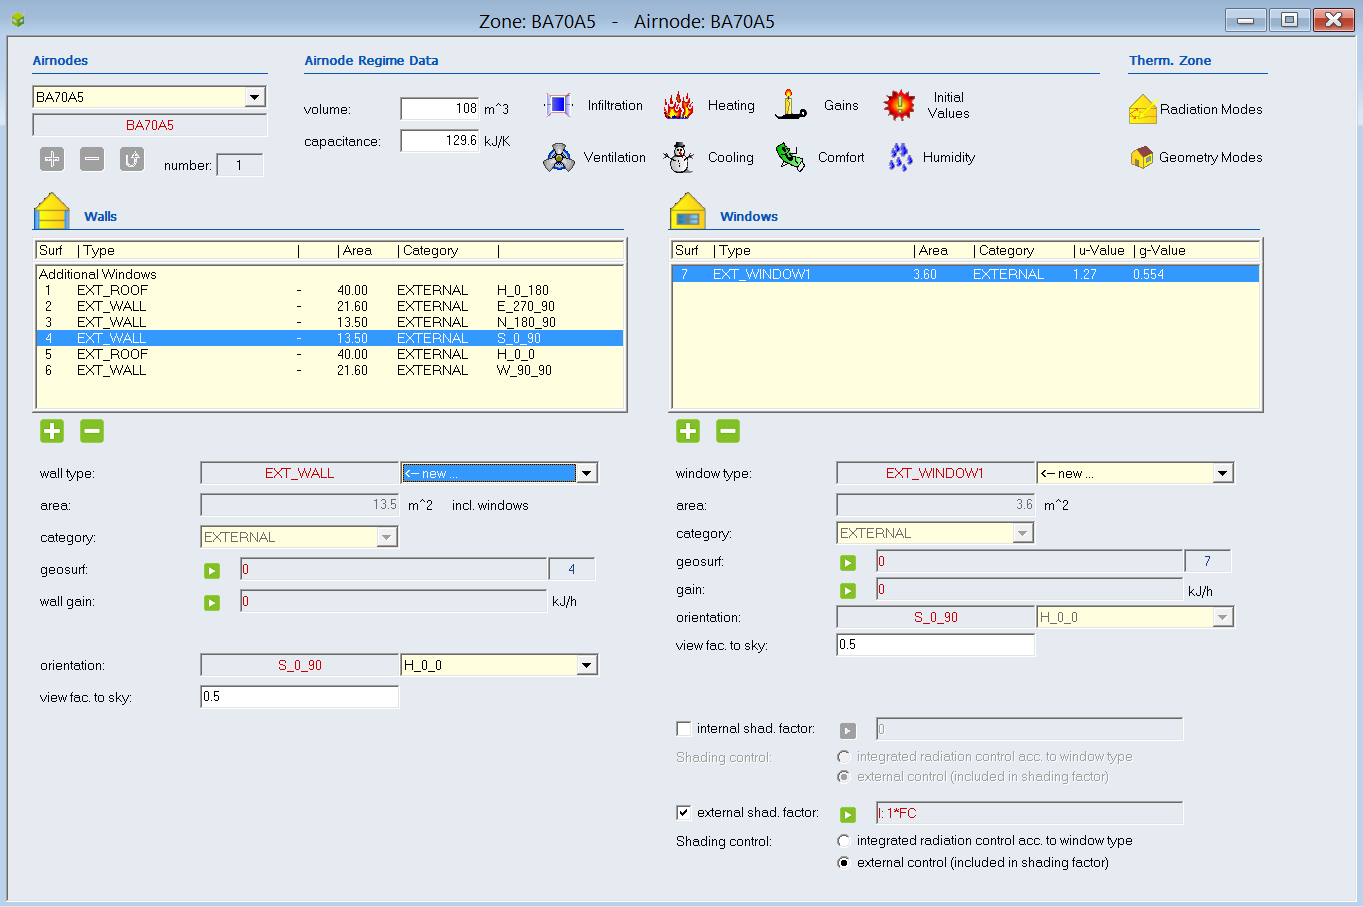
\includegraphics[width=0.7\textwidth]{windowtrnsys}
%\caption{\label{img5:windowtrnsys} Zone window - Fc input as external shading factor}
%\end{figure}
%
%\begin{figure}[h]
%\centering
%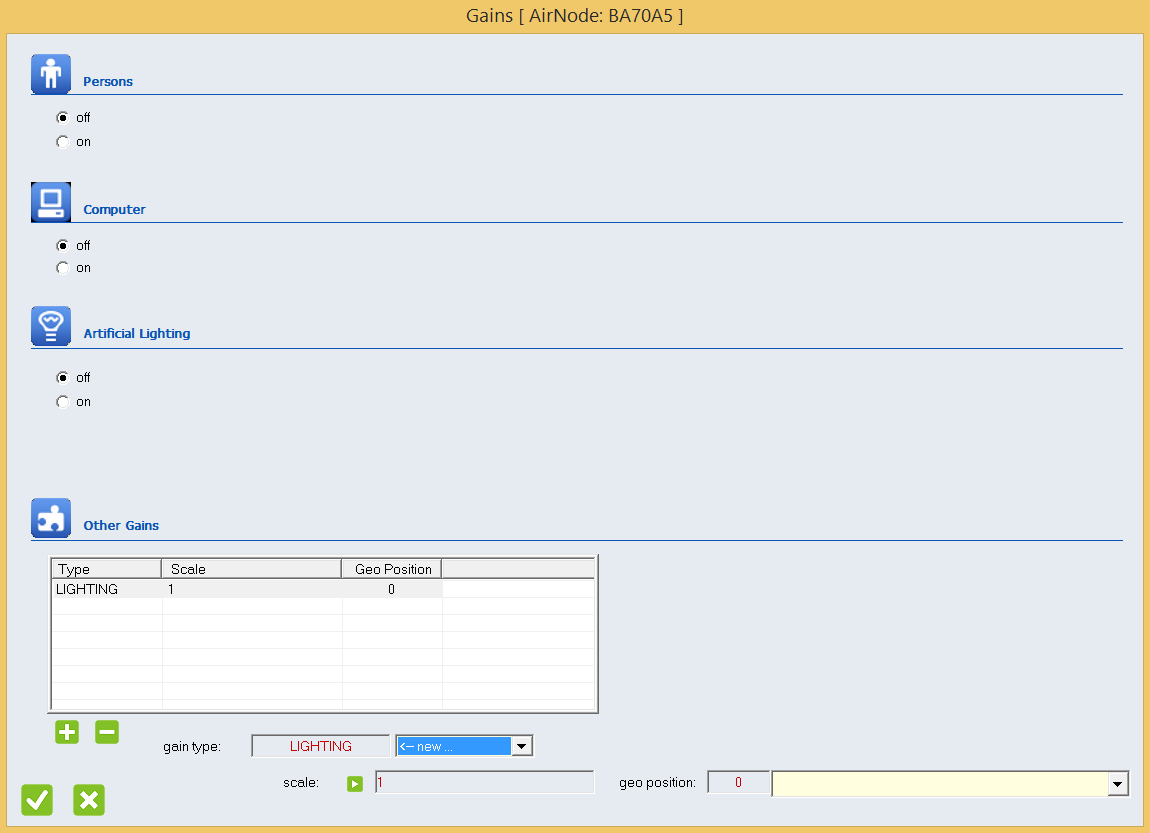
\includegraphics[width=0.7\textwidth]{gain}
%\caption{\label{img5:gain} Gain window - The Artificial lighting gain is considered as Other gain from the TRNSYS deck}
%\end{figure}
%
%The gains due to the artificial lighting are calculated through an ad hoc equation. The equation takes in input the minimum illuminance level over the sensors grid from the TypeDLT and if the natural light is lower than the threshold value of 500 lux the artificial light is dimmed to reach this level. The artificial light power required to arrive at 500 lux is converted in heat gain and passed at each time-step to the Type56 as external gain (Figure \ref{img5:gain}). 





%\printbibliography

\end{document}